\chapter{Background}
\label{chapter2}

I love football \cite{sarmento2014match}

This chapter presents an analysis of the current body of work that serves as the foundation for the PhD thesis on a carbon-neutral dynamic ride-sharing service. It positions the Ride-Sharing problem, its variants and associated challenges, including the optimisation issues connected with ride-sharing, the function of AEVs, the integration of SECs, and the crucial necessity of charging infrastructure. The chapter provides the context for the design, implementation and evaluation of the novel ride-sharing models proposed in subsequent chapters.

\section{The Vehicle Routing Problem (VRP)}
\label{sec:vrp}
This section provides the background necessary to understand the dynamic ride-sharing framework developed in this PhD thesis. Section~\ref{sec:vrp} begins by introducing the classical Vehicle Routing Problem (VRP), outlining its fundamental definitions and common variants. Section~\ref{Section22} then shifts focus to the ride-sharing paradigm, detailing how the VRP can be adapted to transport passengers instead of goods and discussing time-window constraints, routing decisions, and service requirements. Finally, Section~\ref{sec:dynamic} explores the challenges of real-time or dynamic ride-sharing, highlighting the necessity of adaptive routing algorithms that respond to real-time demand uncertainty. Together, these sections establish the theoretical foundation upon which the subsequent chapters of this dissertation will build.

The VRP is a combinatorial optimisation problem that aims to determine the optimal set of routes for a fleet of vehicles to serve a set of customers \cite{pan2023review}. The VRP is extensively studied in operations research and logistics due to its relevance in transportation, delivery, and service operations \cite{maroof2023vehicle}. It was first introduced by Dantzig and Ramser \cite{dantzig1959truck}, as a generalisation of the Traveling Salesman Problem (TSP) presented by Flood \cite{flood1956traveling}. 

The VRP is generally defined on a graph $G = (V, E, C)$, where:
\begin{itemize}
    \item $V = \{v_0, \dots, v_n\}$ is the set of vertices;
    \item $E = \{(v_i, v_j) \mid (v_i, v_j) \in V^2, i \neq j\}$ is the set of edges;
    \item $C = (c_{ij})_{(v_i, v_j) \in E}$ is a cost matrix defined over $E$, representing distances, travel times, or travel costs between the edges.
\end{itemize}

Traditionally, vertex $v_0$ is called the \textit{depot}, while the remaining vertices in $V$ represent customers (or requests) that need to be serviced. 

A solution of the VRP consists of a set of routes for $K$ identical vehicles based at the depot, such that each of the vertices is visited exactly once, while minimising the overall routing distance or travel time or cost. Solving VRP is known to be NP-hard, meaning the computational effort required to find an optimal solution grows exponentially with the problem size. For \( V \) vehicles and \( N \) customers, the number of potential solutions can be expressed as:

\[
\text{Potential solutions} = N! \times \left( \frac{V^N}{V!} \right)
\]

Where:
\begin{itemize}
    \item \( N! \) is the number of ways to arrange \( N \) customers.
    \item \( V^N \) represents the different ways to assign \( N \) customers to \( V \) vehicles.
    \item \( V! \) accounts for the indistinguishability of homogenous vehicles.
\end{itemize}

Figure \ref{fig:vrp_illustration} (resp. Figure \ref{fig:vrptw}) show a subset of possible VRP routes for a problem instance with 2 vehicles and 3 customers (resp. with 3 vehicles and 15 customers). As it can be seen below, the solution space grows exponentially as the number of vehicles and passengers grow linearly: 

\[
\text{Potential solutions} = 3! \times \left( \frac{2^3}{2!} \right) = 6 \times \frac{8}{2} = 24
\]

Figure~\ref{fig:vrptw} extends the scenario to three vehicles and fifteen customers. As the number of vehicles and customers increases linearly, the solution space increases exponentially. The formula remains the same, but plugging in \(V = 3\) and \(N = 15\) yields:
\[
\text{Potential solutions} 
= 15! \times \frac{3^{15}}{3!}
\approx 1{,}307{,}674{,}368{,}000 
\times \frac{14{,}348{,}907}{6}
\approx 3.13 \times 10^{18}.
\]
Thus, even moderate VRP instances can become computationally formidable, highlighting the need for efficient heuristic or approximation algorithms.


\begin{figure}[htbp]
    \centering
    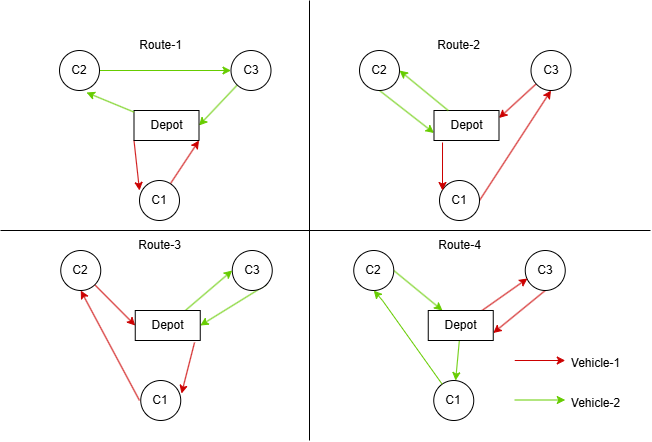
\includegraphics[scale=0.6]{Crest/Images/vrp_illustration.png}
    \caption{A sample of VRP routes with 2 vehicles and 3 customers.}
    \label{fig:vrp_illustration}
\end{figure}

Beyond this standard formulation, VRP has numerous variants \cite{vrp_survey}, including:
\begin{enumerate}
    \item Capacitated VRP (CVRP) in which each customer has a demand for a good and that vehicles have a limited capacity
    \item The VRP with pick-up and Delivery (PDP) in which the goods must be picked up and delivered in a certain amount at each vertex.
    \item  Heterogeneous Fleet VRP (HVRP), in which the vehicles have different capacities.
\end{enumerate}


\section{Ride-Sharing Problem}\label{Section22}
This PhD thesis presents models for a carbon-neutral dynamic ride-sharing service, so it is critical to grasp the concept of ride-sharing first, before exploring dynamic ride-sharing and its challenges. Traditionally, ride-sharing, also called carpooling, is the sharing of journeys so that more than one person travels in a car. It aims to bring travellers with similar itineraries and travel schedules together, which is mostly a commitment among travellers. Ride-sharing provides societal and environmental benefits such as sharing fuel costs, tolls, or other potential travel costs with other travellers, which can lower cost per traveller. It also leads to a reduction in GHG emissions and traffic congestion due to the reduced number of vehicles on the road.

\begin{figure}[htbp]
    \centering
    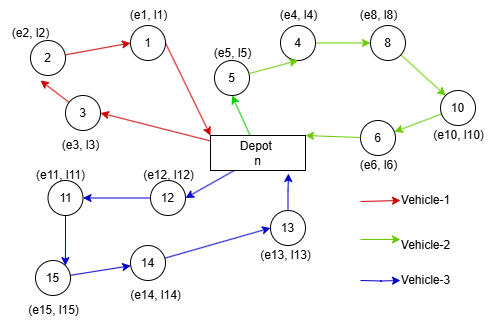
\includegraphics[scale=0.6]{Crest/Images/ride-share_illustration.png}
    \caption{Illustration of a VRP with 3 vehicles and 15 passengers.}
    \label{fig:vrptw}
\end{figure}

The ride-sharing problem combines the VRP with Time Windows (VRPTW) with the Dial-a-Ride Problem (DARP) \cite{paparella2024congestion} where the routing component of the VRP involves the movement of passengers between locations. This preliminary, basic version of the ride-sharing problem is a natural step from the broader VRP to the dynamic ride-sharing context. In this basic formulation, each customer must be visited (even if serving them late violates their designated time window), and all customers are ultimately brought back to the depot. Vehicles may arrive at a location before the designated time window begins; however, service cannot commence until the time window is officially open. In practice, arrivals after the stated time window are often disallowed (hard constraints), but a model may choose to accommodate such late arrivals by imposing penalty costs (soft constraints). In the fully strict or “hard” model, any route that serves a customer outside its time window is infeasible, and that customer would effectively remain unserved. In contrast, a “soft” model permits service outside the window but penalises lateness, ensuring every customer is still visited while acknowledging real-world flexibility in scheduling \cite{soa_rideshare}.

The formulation of the ride-sharing problem is dependent on the objectives and constraints under consideration \cite{asghari2021green}, and is generally defined by: 

\begin{itemize}
    \item A set of identical vehicles denoted by \( K \),
    \item A directed graph network \( G(N, A) \), where:
    \begin{itemize}
        \item \( N \): Set of nodes (customers and the depot),
        \item \( A = \{(i, j) : i \neq j, i, j \in N\} \): Set of vertices or directed routes between nodes.
    \end{itemize}
    \item Node \( 0 \) represents the central depot, while \( N^* = N \setminus \{0\} \) represent customers.
    \item The distance and transit time between two nodes is denoted as \( d_{ij} \) and \( t_{ij} \), respectively. The transit time depends on both static factors (as the distance) and dynamic factors (as the traffic at the given time the distance is traversed). In this PhD thesis, for simplicity of the proposed models, ride-sharing is restricted to static factors only; specifically, the transit time is assumed to be equal to the distance (\( t_{ij} = d_{ij} \)) (i.e., simulating a constant speed for traversing it). This assumption is made to decrease computational complexity and aid in the creation of traceable optimisation models. Incorporating dynamic elements like real-time traffic congestion would need integrating predictive models or real-time data streams, which would greatly increase processing overhead. Furthermore, such dynamic aspects bring unpredictability, making it difficult to obtain reproducible optimisation results. 
\end{itemize}

Each customer \( i \in N^* \) is characterised by:
\begin{itemize}
    \item \( q_i \): Travel Demand of the customer where the demand is pick up point and time and drop of point and time of customer \(i\),
    \item \( s_i \): Service time required at the customer,
    \item \( (e_i, l_i) \): Time window, where \( e_i \) is the opening time, and \( l_i \) is the closing time,
    \item \( a_i \): Arrival time of the vehicle at the customer,
    \item \( w_{ik} \): Waiting time of vehicle \( k \) at customer \( i \).
\end{itemize}

The decision variable \( x_{ijk} \) is defined as:
\[
x_{ijk} =
\begin{cases} 
1 & \text{if vehicle } k \text{ travels from node } i \text{ to node } j, \\
0 & \text{otherwise.}
\end{cases}
\]

Let \( y_i \) is a binary variable such that:
\[
y_i =
\begin{cases} 
1 & \text{if customer } i \text{ is served}, \\
0 & \text{otherwise.}
\end{cases}
\]

In this context, three potential goals for the ride-sharing problem are:

\begin{itemize}
    \item \textbf{Goal 1}: Minimise the total number of vehicles used.
    \item \textbf{Goal 2}: Minimise the total distance travelled.
    \item \textbf{Goal 3}: Minimise the number of customers not being served.
\end{itemize}

An objective function for the ride-sharing problem can be designed to focus on a specific goal or to simultaneously attempt to optimise multiple goals by applying a weight \( W_i \) to each separate goal:

\[
\min \left( W_1 \sum_{k \in K} \sum_{j \in N^*} x_{0j}^k + W_2 \sum_{k \in K} \sum_{(i, j) \in A} d_{ij} x_{ijk} + W_3 \sum_{i \in N^*} (1 - y_i) \right)
\]

In the formula above, \( W_1, W_2, \) and \( W_3 \) are weight factors that determine the priority assigned to each goal in the objective function. It is important to note that the third term maximises the number of TPs served by rewriting it in minimisation form, as minimising \( (1 - y_i) \) effectively maximises \( y_i \), which represents the number of customers served.

\textbf{The set of constraints to be satisfied by any valid solution of the ride-sharing problem is presented below:}
\begin{align}
    \sum_{i \in N} q_i \sum_{j \in N} x_{ij}^k &\leq q_{\text{max}}^k, \quad \forall k \in K \tag{3.1} \\
    \sum_{k \in K} \sum_{j \in N} x_{ij}^k =1, \forall i \in N \tag{3.2}\\
    \sum_{j \in N^*} x_{0j}^k =1, \forall k \in K \tag{3.3}\\
    \sum_{j \in N} x_{ij}^k - \sum_{j \in N} x_{lj}^k &= 0, \quad \forall l \in N, \forall k \in K \tag{3.4} \\
    \sum_{j \in N^*} x_{j0}^k &= 1, \quad \forall k \in K \tag{3.5} \\
    a_0 = w_{0}^k = s_0 &= 0 \tag{3.6} \\
   \sum_{j \in N} x_{ij}^k( a_i + w_{i}^k + s_i + t_{ij}) &\leq l_j, \quad \forall i \in N, \forall k \in K \tag{3.7} \\
    e_i \leq a_i + w_{ik} &\leq l_i, \quad \forall i \in N, \forall k \in K \tag{3.8} \\
    % x_{ij}^k &\in \{0, 1\}, \quad \forall (i, j) \in A, \forall k \in K \tag{3.9} \\
    y_i &\leq \sum_{k \in K} \sum_{j \in N} x_{ij}^k, \quad \forall i \in N^* \tag{3.9}
\end{align}

The constraint (3.1) states that the capacity of the vehicle (\(q_{\text{max}}^k)\) cannot be exceeded and constraint (3.2) that each customer must be served exactly once and by one vehicle. The set of constraints (3.3), (3.4) and (3.5) make sure that each vehicle starts from the depot {0}, visits and serves a certain number of customers, and finally returns to the depot {0}. Constraints (3.6), (3.7) and (3.8) indicate that for a trip from node i to node j, no vehicle may arrive at customer j after the end of the time window, (\(l_i)\). Constraints (3.9) ensures that a customer \( i \) is marked as served (\( y_i = 1 \)) only if there exists a vehicle \( k \) that travels to node \( i \). Simultaneously, the time of arrival to a customer, depends on the time of arrival, the waiting time and the service time, to the previous served customer. 

This MIP model provides a formulation of the general ride-sharing problem, serving as a foundation for more complex variations such as dynamic ride-sharing. An example of an instance for this ride-sharing problem, with 3 vehicles and 15 customers, is illustrated in Figure \ref{fig:vrptw}. The approach taken in Chapter  \ref{chapter3} differs as it incorporates real-time demand uncertainty and adaptability, which are not explicitly captured in this static MIP formulation. The following section delves into these challenges and the proposed solutions for dynamic ride-sharing. 


% \section{Ride-Sharing Services}
% \label{sec:ridesharing}

% Ride-sharing services extend the VRP by introducing paired pickup and drop-off locations for passengers, dynamic requests, and vehicle capacity constraints. This section highlights the unique aspects of ride-sharing compared to traditional VRP.

% \subsection{Concept of Ride-Sharing Services}
% Ride-sharing systems aim to transport multiple passengers efficiently by reducing the number of vehicles on the road, minimizing pollution, and lowering traffic congestion. These systems require vehicles to route dynamically between pickup and drop-off points, ensuring optimal passenger satisfaction while adhering to operational constraints.

% \subsection{Example: Ride-Sharing Problem}
% Consider an instance with 2 vehicles and 3 passengers, where each passenger has a distinct pickup and drop-off location:
% \begin{figure}[htbp]
%     \centering
%     \includegraphics[scale=0.6]{images/ridesharing_example.png}
%     \caption{Illustration of ride-sharing with 2 vehicles and 3 passengers.}
%     \label{fig:ridesharing_example}
% \end{figure}

% While there are multiple ways to route the vehicles, some trip petitions (TPs) may remain unsatisfied due to constraints like vehicle capacity or time windows. For example:
% \begin{itemize}
%     \item Vehicle 1 picks up Passenger A and drops them off but cannot pick up Passenger B due to time constraints.
%     \item Vehicle 2 can pick up Passengers B and C but cannot complete all trips without violating time windows.
% \end{itemize}
% This example highlights the importance of prioritizing TPs and optimizing routes to maximize trips served—a key objective of this PhD.


\section{Dynamic Ride-sharing Problem}
\label{sec:dynamic}
Nowadays, transportation, like many other aspects of daily life is being transformed by the information technology (IT) \cite{golob2001impacts}. The widespread use of mobile devices, as well as the development of the Global Positioning System (GPS), enable all transport operators to adapt transport supply to travel demand in real-time. These possibilities have resulted in the development and evolution of ride-sharing known as dynamic ride-sharing \cite{srinivasan2006impact, altshuler2017ridesharing}.

A dynamic ride-sharing service can be defined as a reactive VRPTW, in which TPs are released over time, while the vehicles may already be en route or stationed at different places \cite{kucharski2017realtime, liao2024towards}. This is distinct from a proactive or static VRPTW, in which all TPs are known in advance. 

To better grasp the dynamic feature of the service, Figure \ref{fig:dynamic_rs_illus} depicts the route execution of a single vehicle satisfying TPs. The vehicle plans an initial route to visit the currently known TPs (A, B, C, D, and E) before it departs the depot (time t0). At time t1, two additional petitions (X and Y) are released, leading to re-route of the vehicle in order to accommodate them. Finally, at time tf, the performed route is (A,B,C,D,Y,E,X).
\begin{figure}[htbp]
    \centering
    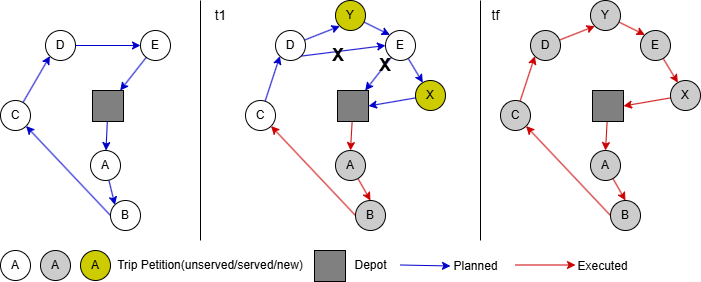
\includegraphics[scale=0.6]{Crest/Images/dynamic_ride_sharing_example.png}
    \caption{Example of dynamic ride-sharing}
    \label{fig:dynamic_rs_illus}
\end{figure}
This example demonstrates how dynamic TPs may lead to re-routing existing vehicles on an ongoing basis, necessitating real-time communication between vehicles and the dispatching centre. Figure \ref{fig:dynamic_routing} depicts a real-time communication example in which the \textit{dispatcher} is the agent that delivers instructions to the vehicle. When the vehicle is ready (first dotted arrow), the dispatcher makes a decision and directs it to complete petition A (first double headed arrow). When the vehicle begins (second dotted arrow) and stops (third dotted arrow) service at petition A, it alerts the dispatcher, who updates the available information and sends the vehicle its next request (second double-headed arrow).
\begin{figure}[htbp]
    \centering
    
\includegraphics[scale=0.6]{Crest/Images/timeline_events.png}
    \caption{Timeline of events for the dynamic routing of a single vehicle}
    \label{fig:dynamic_routing}
\end{figure}

This PhD thesis considers the following key features in order to accommodate dynamic ride-sharing:

\textbf{Time Dimension:} 
The dispatcher must have precise knowledge of the location of all vehicles at any time, in order to respond effectively to service new upcoming TPs or other dynamic information.

% \textbf{Near-Term Events are More Important:} 
% Dynamic routing requires prioritisation of near-term events, as it would be risky to allocate vehicle resources prematurely to long-term requirements. Dispatchers in dynamic scenarios must focus on addressing immediate demands.

\textbf{Information Update Mechanisms are Essential:} 
In dynamic routing environments, system inputs such as new TPs or vehicle availability evolve continuously over time. To maintain solution feasibility, the routing process must incorporate update mechanisms—these refer to procedures or algorithms that periodically or event-drivenly revise vehicle routes, schedules, and resource allocations based on the most recent system state. For example, when a new TP is submitted or an AEV becomes available after completing a task, the routing solution is recalculated to integrate this information. Such mechanisms are unnecessary in static settings, where all system inputs are fixed and known in advance.

\textbf{Re-sequencing and Re-assigning Decisions May Be Warranted:} 
New inputs in dynamic routing can turn previously made decisions as sub-optimal in light of the new context. As a result, dispatchers may need to re-route or re-assign vehicles to adapt to new circumstances and maintain efficiency.

\textbf{Faster Computation Times Are Necessary:} 
In static routing, dispatchers might afford longer computation times to obtain high-quality or even optimal solutions. However, in dynamic scenarios, dispatchers most likely need to generate solutions quickly (perhaps within minutes or seconds) in order to address the immediate problem. This time constraint often necessitates the use of local improvement heuristics, such as insertion and \(k\)-interchange, for re-routing and re-assignments.
Local improvement heuristics are a class of optimisation techniques designed to refine existing solutions by making small adjustments iteratively \cite{cordeau2007dial, gendreau1994tabu}.  
\begin{itemize}
    \item \textbf{Insertion Heuristic}: This method involves inserting a new request (or modifying an existing one) into an existing route in a way that minimises additional cost. It evaluates various potential insertion points and selects the one that results in the least disruption to the current schedule \cite{jaw1986heuristic}.
    \item \textbf{\(k\)-Interchange Heuristic}: This heuristic swaps up to \(k\) requests between different routes to improve overall efficiency. By exchanging a subset of trips between different vehicles, the method aims to balance loads, reduce travel time, or optimise service times \cite{potvin1993kinterchange, berbeglia2010dynamic27}.
\end{itemize}
These heuristics enable dispatchers to generate feasible solutions in real-time, making them particularly useful in dynamic routing scenarios where computational speed is critical.

\textbf{Objective Functions in Dynamic Settings May Differ from Those in Static Routing Problems:} 
In conventional static vehicle routing or ride-sharing models, objective functions often focus on minimising total travel distance, total service time, or the number of vehicles used, with all trip demands known in advance. However, in dynamic ride-sharing environments where TPs are continuously generated, vehicles are reallocated in real-time, and system states evolve unpredictably, such static objectives may lose relevance. Optimisation strategies in such contexts must operate on partial information, incorporating real-time data and, where possible, probabilistic estimations of future events to ensure effective service performance \cite{spall2003introduction}.

\textbf{Time Constraints May Be More Flexible:} 
In dynamic routing problems, time constraints such as latest pickup times are often more flexible than in static problems. Denying service to an imminent demand due to a minor breach of time constraints is generally less desirable than accommodating the request by relaxing these constraints \cite{ichoua2003vehicle}.

\textbf{Centralised vs Decentralised Approaches:} In a centralised system, a central unit collects and processes all \cite{alonso2017demand}, adding to the complexity of the dynamic ride-sharing problem. In a decentralised system, the vehicle itself or an aggregator could process some of the information. This depends on the ride-sharing fleet provider and is explored further in the following section.

% \begin{enumerate}
%     \item \textbf{Time Dimension is essential:} In a static routing problem, the time dimension may or may not matter. In a dynamic counterpart, time is always important. In response to service requests or other information, the dispatcher must know the location of all cars.

%     \item\textbf{Near-term events are more important:} BeIn a static routing problem, all events receive equal weight due to the homogeneity of information quality and the absence of input updates. In a dynamic situation, it would be imprudent to quickly devote vehicle resources to long-term requirements. When dealing with a dynamic routing problem, the dispatcher should prioritise near-term events.

%     \item\textbf{Information update mechanisms are essential:} Almost all inputs to a dynamic routing problem can alter during the day of operation. It is consequently necessary to incorporate information update techniques into the solution procedure. Naturally, information update techniques are irrelevant in a static setting.

%     \item\textbf{Re-sequencing and reassigning decisions may be warranted:} In dynamic routing, fresh input may cause the dispatcher's decisions to become suboptimal. This causes the dispatcher to reroute or even reassign vehicles in order to address the new scenario.

%     \item\textbf{Faster computation times are necessary:} In static settings the dispatcher may a ord the luxury of waiting for a few hours in order to get a high quality solution, in some cases even an optimal one. In dynamic settings this is not possible, because the dispatcher wishes to know the solution to the current problem as soon as possible (preferably within minutes or seconds). The running-time constraint implies that rerouting and reassignments are often done by using local improvement heuristics like insertion and k-interchange.

%     \item \textbf{Indefinite deferment mechanisms are essential:} Indefinite deferment refers to the possibility that the service of a certain demand may be postponed indefinitely due to the demand's unfavourable geographical qualities in comparison to the other demands. This problem could be solved by employing time window constraints or a nonlinear objective function that penalises excessive waiting.

%     \item \textbf{Objective function may be different:} Traditional static objectives, such as minimising total distance travelled or overall schedule duration, may be meaningless in a dynamic situation where the process is open-ended. If no knowledge about future inputs is available, it may be appropriate to optimise just over known inputs. Some services employ nonlinear objective functions to avoid unwanted events such as the aforementioned infinite deferment.

%     \item\textbf{Time constraints may be different: } Time limitations, such as the latest pickup times, are softer in dynamic routing problems than in static ones. This is owing to the fact that denying service to an imminent demand if the time constraint is not satisfied is typically less appealing than breaching it.
% \end{enumerate}

% In summary, dynamism can be defined as:
% \begin{itemize}
%     \item A problem is dynamic if its parameters change over time. This includes models with dynamic data that change constantly as well as problems with time-dependent data that are known in advance.

%     \item A model is dynamic if it explicitly incorporates the interaction of activities over time. Here one should distinguish between deterministic dynamic models and stochastic models.

%     \item If an application solves the underlying model repeatedly as new information comes in, it is considered dynamic.Subsequently, solving models within dynamic applications requires huge computational resources.
% \end{itemize}

The primary components of the dynamic ride-sharing service are the passenger, vehicle, and matching algorithm. The passenger seeks a ride that will pick her/him up at the starting place and drop her/him off at the desired destination within a time frame. The transportation provider has a fleet of vehicles (taxi, van, autonomous vehicle, etc.) ready to satisfy the needs of a passenger. The matching and routing algorithm gets requests and fleet information and attempts to find the best matches on short notice. As co-operation/collaboration between different fleet providers is critical for this PhD thesis and the models it proposes, the different key aspects defining such potential co-operation/collaboration are described in Figure \ref{fig:rideshare_category}. Fleet providers can operate either competitively or cooperatively. In a competitive planning approach, fleet providers are competitors, and they hesitate to share information about their cost structures and TPs  \cite{agatz2012optimization}. Relying on a neutral dispatcher to re-assign jobs within the system establishes the compensation and profit sharing framework. These scenarios are referred to as centralised competitive planning approaches. On it, a neutral, centralised dispatcher attempts to address the whole set of TPs, notifying each fleet provider of the ones assigned to it \cite{agatz2012optimization}.

\section{Decentralised Dynamic Ride-sharing }
\label{sec:decentralised}

In the case of cooperative interaction, providers exchange fleet information, making it easier for the passenger to get a ride and increasing the benefits of ride-sharing \cite{shen2018integrating}. For a decentralised approach, the fleet providers have to reveal only a small proportion of the information they would have to disclose in a centralised approach \cite{klapp2020decentralized}. For instance, in a centralised system, fleet providers must share their complete availability, pricing structures, and operational constraints with a central authority, which can lead to concerns over data privacy, competition, and strategic disadvantages. In contrast, a decentralised approach allows fleet providers to retain autonomy by only disclosing essential details such as available capacity or general service regions, reducing information overhead while maintaining independence. This PhD thesis focuses in both centralised and decentralised approaches for cooperative ride-sharing. In both cases, the effectiveness of the system relies on the matching and routing algorithm allowing to maximise the trips served.

A dispatcher receives the TP info from each passenger. It also gets access to the fleet being able to monitor the position, route and passenger allocation of each vehicle at any given time. The system processes the passenger TPs as they arise, potentially re-routing an existing vehicles to pick up and drop off the new passenger as requested \cite{masoud2017decentralized}. Despite the limited practical use of centralised collaborative approaches, due to trust issues, solving the centralised problem remains critical for this PhD thesis, even if only as a benchmark for its comparison with counterpart decentralised approaches. 

Figure \ref{fig:collaborative} illustrates a scenario with and without collaboration (respectively top and bottom of the figure) for a routing problem involving three carriers. The figure is based on equal workloads, meaning each vehicle tries to serve an equal number of TPs. 

\begin{figure}[htbp]
    \centering
    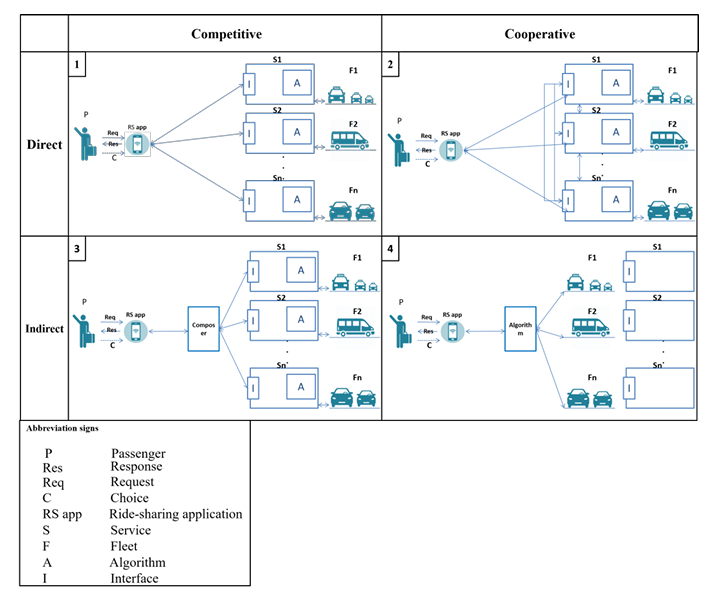
\includegraphics[scale=0.6]{Crest/Images/dynamic_rideshare_category.png}
    \caption{Different categories of dynamic ride-sharing \cite{soa_rideshare}}
    \label{fig:rideshare_category}
\end{figure}

In the collaborative scenario (bottom part of the figure), carriers are able to exchange TPs, leading to a more efficient overall allocation of resources. This results in shorter total travel distances, reduced vehicle idle time, and more balanced route distributions across the carriers. The exchange of requests allows each vehicle to focus on a more geographically compact set of requests, which reduces unnecessary detours and increases overall service efficiency. 

In contrast, in the non-collaborative scenario (top part of the figure), each carrier is limited to serving only its originally assigned requests, which leads to longer and less efficient routes. Some carriers may end up with routes that have excessive travel distances, while others might experience underutilisation. 

It is evident that every carrier would significantly benefit from these exchanges as they reduce operational costs, improve service times, and create a more balanced workload distribution among the fleets. The models show in chapters \ref{chapter4} and \ref{chapter5} of this PhD will be based on such these collaborative setting.

\begin{figure}[htbp]
    \centering
    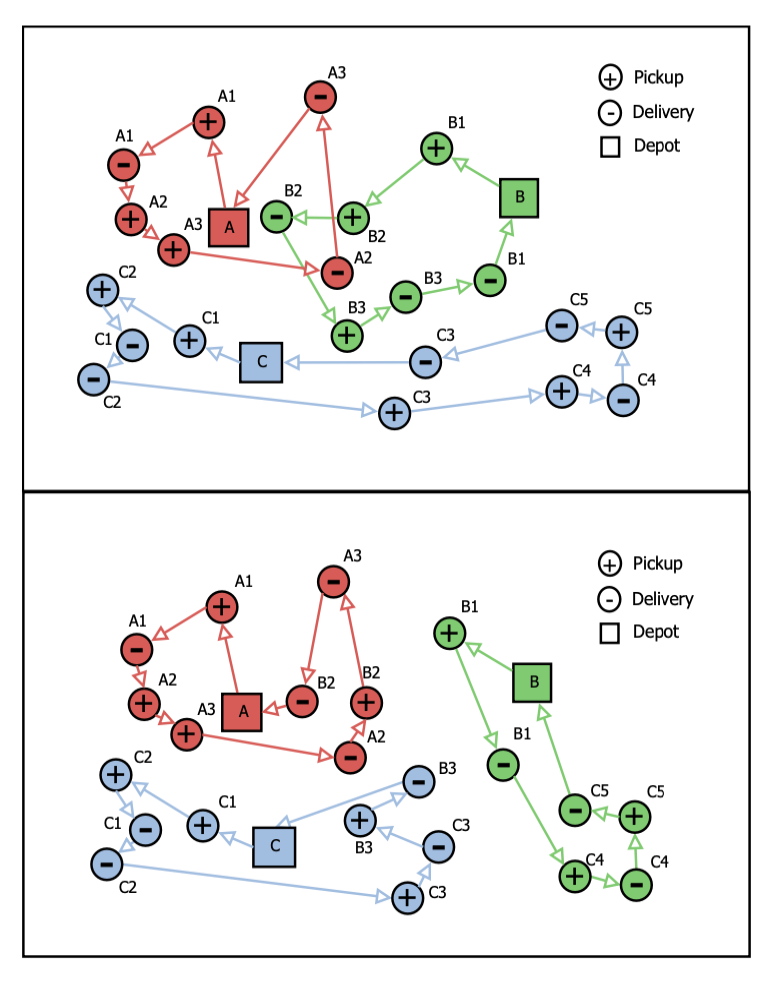
\includegraphics[scale=0.6]{Crest/Images/collaborative_routing.png}
    \caption{Example of non-collaborative planning(top) and collaborative(bottom) planning}
    \label{fig:collaborative}
\end{figure}

\section{Autonomous Electric Vehicles (AEV)}
\label{sec:aevs}
Another significant innovation that has the potential of impact ride-sharing services in the coming decades is the introduction of Autonomous Electric Vehicles (AEVs). 
The following definition by the author \cite{fagnant2014future} represents the term “Autonomous Vehicle” (AV) as used in this PhD thesis:
\textit{Autonomous vehicles are vehicles that can drive without human intervention or monitoring in an unpredictable, uncertain, and open traffic environment designed, built, and populated by and for humans. It represents the highest level of autonomy and thus the ideal future end-state of these vehicles.} 

One of the challenges associated with ride-sharing is the limitations faced by a vehicle due to the availability of its owner to drive it. Incorporating AEVs into the system would prove instrumental in removing these limitations (allowing each vehicle for 24/7 service) while also reducing emissions, enhancing street safety, saving time and space, and reducing congestion. The PhD thesis focuses on using AEVs for ride-sharing for the above-mentioned reasons.

\section{Smart Energy Communities (SECs)}
\label{sec:secs}

The ride-sharing models proposed in this PhD thesis are based on the use of SECs. These can be defined as: (1) AEV depots, (2) cooperative dispatchers, and (3) localised energy hubs. The SECs represent the solely source for charging the AEV fleet of the ride-sharing service. Specifically, they make the service carbon-neutral, by using solely the RES generated by each SEC (e.g., solar and wind power) to charge the vehicles \cite{paranjape2020urban}. By restricting itself to operate under 100\% RES, the SECs-based ride-sharing service often face resource constraints. For example, on a given day, one of the SECs of the ride-sharing service owning a total of 10 AEVs, may only generate enough energy to charge 5 of them during peak ride-sharing service hours (therefore not being able to use the other 5 EVs at all, which remain idle at the SEC depot). It is in the context of this resource scarcity that the ride-sharing service will benefit from the intelligent scheduling and resource allocation models proposed in this PhD thesis.

A key feature of SECs is their ability to engage in cooperative strategies with neighbouring SECs, enabling shared resource utilisation \cite{peterson2020integrating}. However, to ensure effective cooperation, the challenges such collaboration introduce must be addressed, including:
\begin{itemize}
    \item \textbf{Efficient Fleet Allocation:} Determining which EVs to dispatch and where, without disrupting local operations.
    \item \textbf{Equitable Reward Mechanisms:} Designing incentives that fairly compensate SECs for contributing resources while fostering long-term collaboration.
    \item \textbf{Real-Time Decision Making:} Adapting to dynamic demand and energy availability in real-time while minimising computational delays.
    \item \textbf{Sustainability Trade-offs:} Balancing operational efficiency with carbon-neutral objectives, especially when collaboration may increase travel distances for EVs.
\end{itemize}

As an example of the benefits of such collaborations, suppose SEC A has a fleet of AEVs primarily serving TPs within its region, but it receives an unusually high demand for rides due to a local event. Meanwhile, SEC B, located nearby, has surplus fleet capacity because its demand is relatively low at the same time. The two SECs can then negotiate a fleet allocation arrangement:
\begin{itemize}
    \item \textbf{Negotiation Terms:} SEC A can request a SEC B to dispatch a number of its AEVs to serve some of the TPs SEC A is facing. In return, SEC A offers to compensate SEC B with either charging credits at its AEV charging facilities and/or with the promise of future fleet assistance on a potential future time peak demand period for SEC B.
    \item \textbf{Outcome:} A number of AEVs from SEC B temporarily operate serving some of the TPs SEC A is facing reducing unmet trip demand in SEC A while ensuring such AEVs from SEC B remain operationally utilised rather than idle. This negotiation dynamically balances resource utilisation across SECs, improving the overall service efficiency of the ride-sharing service.
\end{itemize}

This example underscores how negotiation and incentive systems between SECs can address demand fluctuations and resource constraints. The ride-sharing network enhances its overall efficiency by carrying out inter-SEC negotiations leading to dynamically re-allocation of AEVs. These mechanisms contribute to the efficiency of the ride-sharing service, specially in light of the aforementioned carbon neutrality restrictions. Further discussions on the design and implementation of these collaborative strategies are provided in chapters \ref{chapter4} and \ref{chapter5}. To the best of our knowledge, this is the first study that leverages SEC in this context to build a carbon-neutral dynamic ride-sharing service. 

\section{Charging Infrastructure}
\label{sec:charging}

Integrating AEVs into ride-sharing introduces several challenges, such as restricted battery capacity and downtime during charging operations. These issues are especially significant in the context of the aforementioned carbon-neutral, AEV and SECs-based ride-sharing service described in this PhD thesis, where efficient charging solutions are critical to minimising downtime, ensuring AEV availability, and ultimately maximising the number of trips served. 

To address these challenges, this PhD thesis incorporates strategies for managing AEV charging infrastructure where AEVs are charged at its home SEC, using its locally generated RES available at the time of charging.
Alternatively, an AEV can also charge at a neighbouring SEC, through resource sharing agreements between the host and home SECs as the ones aforementioned described.

Determining the optimal placement for a network of charging stations is a complex problem which is outside the scope of the PhD thesis. In its simplest form, the problem can be modelled as a \textit{facility location problem} \cite{ortiz2018multi}, where the goal is to identify the best locations for AEV depots that also function as charging stations. Alternatively, when a charging station location is interdependent with the routing of the AEVs it hosts, the problem becomes a \textit{location routing problem} \cite{ortiz2018multi}. Planning charging stops within a dynamic ride-sharing service introduces additional complexity due to several interrelated factors. Firstly, the dynamism of ride requests leads to rapidly changing demand patterns, requiring real-time adjustments in vehicle routing and charging schedules. Secondly, time window constraints limit the time during which AEVs can service trips or reach charging stations, necessitating precise coordination to avoid delays or missed requests. Lastly, the need to balance energy availability and trip demands within the network further complicates scheduling, as vehicles must strategically allocate charging opportunities without compromising service efficiency.

The optimisation challenge faced in this PhD thesis is to, given (1) a static network of charging stations (each of them belonging to one of the SECs of the ride-sharing service), (2) a number of AEVs owned by the SECs and (3) a number of TPs, each of them with a weight indicating its importance, decide the schedule of the charging of the AEVs fleet, in such a way it maximises the overall weight of the TPs being served.

To illustrate the challenge, consider the following scenario, where SEC A:

\textbf{Scenario}, SEC A operates a fleet of 10 AEVs, supported by solar panels generating 50 kWh of renewable energy daily. Each AEV requires 60 kWh for a full charge, enabling 100 km of travel. Due to high demand, SEC A needs to prioritise which AEVs are to be charged in order to maximise trip fulfillment. This challenge differs when tackled in the context of AEVs solely charged by their home SECs vs. the context of different SECs negotiating and, therefore, cooperating in the AEVs charging. Each scenario is discussed separately below:

\textbf{Charging Process at Home SEC:} SEC A schedules its charging operations by prioritising those AEVs with a planning route containing the most significant TPs, but resulting in risk of running out of battery if more TPs are added to their route. For instance, EV 1, with 20\% battery, is scheduled for immediate charging to ensure availability for an upcoming ride request. On the other hand, EV 2, with 60\% battery, is placed in a lower priority queue since it is much more likely to be able to accommodate at least one more trip before requiring a battery charge.

\textbf{Charging at Neighboring SECs}: During peak demand, SEC A negotiates with SEC B to charge some of its AEVs. For instance, if an AEV is low on battery and located closer to SEC B than SEC A, it charges at SEC B instead. In return, SEC A compensates SEC B with energy credits or other incentives, ensuring efficient energy distribution and reducing strain on individual SECs.

As a result, such collaborative charging mechanisms help to:
\begin{itemize}
    \item Maximise AEV utilisation by reducing the time spent travelling to a charging station. In the example above, SEC A can serve additional TPs by focusing its local resources on more urgent charging needs.
    \item Enhance the flexibility of the ride-sharing network, allowing SECs to handle peak demands efficiently.
    \item Contribute to the carbon neutrality of the ride-sharing service by optimising the use of RES across SECs.
\end{itemize}

This PhD thesis designs, implements and evaluates models to address the optimisation challenges outlined above, ensuring efficient scheduling of charging operations while maintaining SEC collaboration. Chapter \ref{chapter5} details these solutions, including real-time scheduling strategies and dynamic incentive mechanisms to foster inter-SEC cooperation.

\section{Literature Review}
\label{sec:literature_review}
This section examines the existing literature on dynamic ride-sharing, vehicle fleet allocation, and charge scheduling. The primary goal is to review existing work, so as to better position the specific contributions and challenges addressed by the ride-sharing models proposed in this PhD Thesis.

\section{Dynamic Ride-sharing}
Dynamic ride-sharing involves real-time matching of TPs with available vehicles while optimising fleet utilisation. Unlike static ride-sharing, where routes are planned in advance, dynamic ride-sharing solutions must continuously adapt to new requests, cancellations, and fluctuating demand. Widely studied in operations research and transportation literature [101], the complexity of the problem arises from its multiple constraints and objective functions, which has lead to a number of solution methods to tackle it \cite{meng2021dynamic}.

\subsection{Constraints and Objective Functions}
\label{objectives_constraints}
The constraints and objective function determines the variant of the dynamic ride-sharing problem being considered. Table \ref{table:problem_inputs} surveys the existing literature to classify the constraints and objective functions being considered.

\begin{table}[htbp]
\centering
\renewcommand{\arraystretch}{1.2} 
\setlength{\tabcolsep}{4pt} 
\small 
\begin{adjustbox}{max width=\textwidth}
\begin{tabular}{|p{3.5cm}|p{11cm}|}
\hline
\textbf{Category}            & \textbf{Key Attributes} \\ \hline

\multirow{1}{3.5cm}{\textbf{Transportation Demand}} 
& Time-dependent demand, real-time trip hailing, authentication system, trip motivation, origin, destination, seat demand, maximum waiting time, maximum travel time, maximum detour, maximum fare, time window, desired pick-up and drop-off times, delay tolerance, sharing limit, distance from origin to pick-up, departure time, arrival time. \\ \hline

\multirow{1}{3.5cm}{\textbf{Transportation Service}}
& Vendors, fixed fleet, timetables, fixed stops, waiting locations, homogeneous/heterogeneous vehicle fleet, professional vs. non-professional supply, vehicle capacity, pricing schemes. \\ \hline

\multirow{1}{3.5cm}{\textbf{Algorithmic Considerations}} 
& Objective function, dispatching, searching, scheduling, monitoring, shortest path computation, empty vehicle behaviour, accept/reject TPs, traffic considerations. \\ \hline

\end{tabular}
\end{adjustbox}
\caption{Problem attributes considered in dynamic ride-sharing}
\label{table:problem_inputs}
\end{table}

\textbf{Objective Functions}: In terms of the desired goal, most approaches aim to find the near-optimal solution to the matching problem in ride-sharing services by considering specific objective functions, such as minimising the total travel distance or time \cite{ota2017stars135, qian2017optimal143, dorey2014ridesharing53} and maximising the match between vehicles and passengers \cite{stiglic2016making162, ma2013tshare118, goel2017optimal68, herbawi2012ridematching80, berbeglia2012hybrid28, stiglic2015benefits161, santos2015taxi152} and minimising the number of required vehicles \cite{kirchler2013granular96, lehuede2014multicriteria107}, or vehicle emissions \cite{atahran2014multicriteria22}. 

Travel duration and distance are crucial factors for travellers \cite{naoum2015stochastic133}. Real-time approaches, like \cite{delling2009engineering}, efficiently compute the shortest path in real time. Non-real-time techniques, such as the proposed method in T-Share \cite{ma2013tshare}, can estimate the distance of the shortest path by partitioning the street network into grid cells and determining the shortest path for each anchor node (the nearest node in the road network to the geographical centre). 

Another significant goal for passengers is to minimise the amount of time they have to wait for their journey. Typically the primary aim of passengers is to save money on their trip. According to \cite{stiglic2016making162}, if no match is identified within a certain time frame, passengers are more likely to abandon the system and refuse to use shared mobility services. Minimising total passenger trip or waiting time may improve performance for passengers, but not for the system as a whole. Reducing passenger wait time can make shared services comparable to typical taxi services. Various techniques in the literature strive to decrease the waiting for passengers as an objective function, such as \cite{hyland2018sharing87, kirchler2013granular96, masoud2017using126}. Much of the research on dynamic ride-sharing services focusses on a single provider. These studies typically incorporate restrictions for the problem to retain the passengers aim at an appropriate level \cite{molenbruch2017typology128, calvo2004distributed38}. Theses studies do not take into account multiple objectives unlike the one presented in this PhD thesis, where maximising trips served by using only the available RES is set as a hard constraint.  

In \cite{dorey2014ridesharing53}, total travel distance, taxi stand departures (number of exits from all taxi stands), and revenue per travel distance (revenue per km earned by all vehicles) were used to measure the performance of a vehicle owner in terms of operation mode and costs for all trips. The percentage of served requests, waiting time, journey time, and trip fee are used to determine the preferences of the passengers'. In \cite{kirchler2013granular96}, the authors included six objectives: Routing costs, excess ride time, passenger waiting time, route durations, early arrival times at pickup and delivery nodes, and the number of unfulfilled requests are all minimised.

% \subsubsection{Problem Constraints Categories}
% \label{problem_constraints}
\textbf{Constraints: }In the ride-sharing problem, a set of constraints and features must be taken into account for both transportation demand and transportation service. The constraints of the dynamic ride-sharing problem can be classified into four main categories:

\textbf{Assignment Constraints} ensure that each passenger is assigned to exactly one vehicle and that each trip follows the correct sequence from pick-up to drop-off \cite{stiglic2018enhancing163, goel2017optimal68}. Assignment constraints are the first restrictions of a ride-sharing problem and as a result, assignment limitations are hard constraints that must be satisfied when solving a ride-sharing problem. This has been modelled using a variety of ways in literature. In \cite{stiglic2018enhancing163}, the authors define an intermediary site called a meeting point for passenger pickup or drop off. They show that this meeting place can result in shorter detours. In \cite{goel2017optimal68}, the authors propose a ride-sharing approach where pick-up/drop-off locations are chosen from a fixed set. They describe a strategy for selecting ideally fixed Pick Up Points (PuPs) with the goal of maximising car occupancy rates while maintaining user privacy and safety. In \cite{naoum2015stochastic133}, the drop-off place is a common destination such as a university or company. Other studies focus on supplying passengers door-to-door in order to provide better comfort for sharing participants. In \cite{ota2017stars135, li2016share110, tachet2017scaling165}, passengers can specify pick-up and drop-off locations. In \cite{dorey2014ridesharing53, farin2016framework56, kleiner2011mechanism98}, the pick-up point is the current position of the passenger, and the only location specified is a trip destination.

\textbf{Synchronisation Constraints} maintain consistency in passenger transfers and ensure that multi-leg trips align with scheduling requirements \cite{fink2019column58, drexl2012synchronization54}. Synchronisation constraints are particularly relevant in dynamic ride-sharing systems where passengers may need to transfer between vehicles or where fleets are managed across different providers. In such scenarios, ensuring the coordination of pick-up and drop-off times between dependent trips is essential to avoid excessive waiting times and service disruptions \cite{masoud2017using126, lazzaretti2021real}. 
Beyond passenger transfers, synchronisation constraints also apply to energy constraints in electric vehicle-based ride-sharing services. Vehicles may need to synchronise their trips with available charging opportunities to ensure uninterrupted service, a challenge explored in depth in Chapter \ref{chapter5}.

\textbf{Time Window Constraints} require that passengers are picked up and dropped off within acceptable time limits. In some models, soft constraints allow minor violations with penalty costs \cite{agatz2011dynamic7, naoum2015stochastic133}, but must of the literature on ride-sharing considers the time windows as hard constraints. TSuch time windows are defined using various ways: In \cite{agatz2011dynamic7}, the passenger sets the earliest departure time and time flexibility, which is the difference between the earliest departure time and the latest arrival time. In \cite{naoum2015stochastic133, wang2018stable173, herbawi2012ridematching80, agatz2011dynamic7}, passengers specify the earliest and latest pick-up and arrival times. As a result, the passenger shall be picked up at the origin point no sooner than the specified pick-up time and left off at the destination before the latest arrival time. In \cite{linares2016simulation87}, travellers face implicit rather than explicit time limitations, and the objective function solely takes into account passenger waiting times.

\textbf{Capacity Constraints} restrict the number of passengers assigned to a vehicle based on its seating capacity. Some research aim to utilise the full capacity of the vehicle \cite{goel2017optimal68, dorey2014ridesharing53}. In addition to limiting the maximum number of passengers, studies on van-pooling systems set a minimum number of passengers to create a van-pool for a shared trip \cite{kaan2013vanpool93}. 

In this PhD thesis, capacity constraints are particularly relevant due to the integration of AEVs within SECs. Unlike conventional ride-sharing services that can dispatch additional vehicles when demand spikes, SEC-based ride-sharing services operate under RES constraints, which limit the number of AEVs available at any given time. As a result, it is critical to maximise vehicle occupancy while ensuring that capacity of each AEV is fully utilised to minimise the number of unserved TPs \cite{stiglic2018enhancing163, liu2020optimizing}.

Moreover, in SEC-based ride-sharing, capacity constraints must also consider energy availability. If the battery level of an AEV is low and charging resources are limited, the number of passengers that can be served on a single trip must be carefully managed to ensure that the vehicle can complete its route without requiring an unscheduled recharge \cite{hu2020electric}. This introduces a dual-layered capacity constraint, where both passenger occupancy and battery capacity influence the availability of the vehicles for ride-sharing.

Additionally, ride-sharing services operating with fleet collaboration mechanisms must incorporate fleet-wide capacity management. If an SEC cannot fulfil a ride request due to local vehicle shortages, it may dynamically allocate ride requests to neighbouring SECs. However, this requires strict coordination of available vehicle capacities across multiple SECs while maintaining service efficiency \cite{yang2021dynamic}.

This PhD thesis addresses these capacity constraints by developing an optimisation model that dynamically assigns vehicles based on real-time demand and energy availability. The model prioritises high-occupancy ride matches while ensuring that AEVs remain operational under energy constraints. The methodology and detailed formulation of this model are presented in Chapter \ref{chapter5}.

Table 2.2 provides a structured overview of the primary constraints considered in the literature for dynamic ride-sharing services. It is important to highlight that all these constraints are incorporated within the optimisation models proposed in this PhD Thesis.

While some prior studies incorporate energy constraints, they primarily address vehicle battery capacity or charging limitations in isolation, often assuming access to a static or grid-based energy supply. Unlike such approaches, this PhD thesis explicitly models the impact of renewable energy availability within SECs on ride-sharing feasibility. The energy constraints in this work are directly linked to the fluctuating, decentralised generation profiles of SECs, affecting vehicle dispatch, scheduling, and fleet coordination in real-time. This integrated approach ensures that both transportation and energy resources are jointly optimised, with the objective of maximising the number of trip petitions served under renewable energy constraints.


\begin{table}[ht]
\centering
\label{tab:constraints_table}
\renewcommand{\arraystretch}{1.5}
\resizebox{\textwidth}{!}{%
    \begin{tabular}{|l|c|c|c|}
        \hline
        \textbf{Constraint Type} & \textbf{Relevant Studies} & \textbf{Energy Constraint} & \textbf{Included in This PhD}  \\ \hline
        Assignment   & \cite{stiglic2018enhancing163, goel2017optimal68, naoum2015stochastic133, ota2017stars135, li2016share110, tachet2017scaling165, dorey2014ridesharing53, farin2016framework56, kleiner2011mechanism98} & No & Yes  \\ \hline
        Synchronisation & \cite{fink2019column58, drexl2012synchronization54, tachet2017scaling165, farin2016framework56, goel2017optimal68, masoud2017using126, lazzaretti2021real} & No  & Yes  \\ \hline
        Time Window   &  \cite{agatz2011dynamic7, naoum2015stochastic133, wang2018stable173, linares2016simulation87, herbawi2012ridematching80, agatz2011dynamic7} & No  & Yes \\ \hline
        Capacity  & \cite{goel2017optimal68, dorey2014ridesharing53, tachet2017scaling165, stiglic2018enhancing163, liu2020optimizing, hu2020electric, yang2021dynamic} & Battery Capacity / Charging Limits only  & Renewable Energy-Aware Fleet Coordination \\ \hline
    \end{tabular}%
}
\caption{Summary of problem constraints in dynamic ride-sharing. While some studies address energy constraints such as battery capacity or charging requirements, this PhD uniquely incorporates renewable energy availability from decentralised sources (SECs) into vehicle coordination and ride-sharing feasibility.}
\end{table}



\subsection{Solution Methods}
\label{solution_methods}
Solving the dynamic ride-sharing problem requires a balance between computational efficiency and solution quality. The complexity of the problem stems from its NP-hard nature, meaning that exact solutions become computationally intractable for large-scale instances.To address this, three primary solution approaches are explored in the literature: Exact methods, Heuristics, and Metaheuristics.
\begin{itemize}
    \item Exact Methods: These methods, provide optimal solutions but are computationally expensive. They are mainly used for small problem instances \cite{cordeau2007dial46, ropke2009branch148}. Exact approaches include:
    \begin{enumerate}
        \item \textbf{Mixed Integer Programming (MIP):} Formulates ride-sharing as an integer optimisation problem, typically solved using commercial solvers like CPLEX or Gurobi \cite{cordeau2007dial46, ropke2009branch148}.
        \item \textbf{Branch-and-Bound}: Systematically explores the solution space by pruning suboptimal solutions \cite{cordeau2007dial46}.
        \item \textbf{Branch-and-Cut}: An extension of Branch-and-Bound that includes cutting plane techniques to improve computational efficiency \cite{ropke2009branch148}.
        \item \textbf{Column Generation}: Used in large-scale formulations to iteratively generate variables that improve solution quality \cite{ghilas2018branch65}.
    \end{enumerate}
    
    \item Heuristic Methods: These methods offer computationally efficient alternatives by finding near-optimal solutions within reasonable time frames. These methods are particularly effective for large-scale ride-sharing instances.In general, heuristic approaches rely on one or more of the following criteria to dynamically make decisions without further reconsidering them:
    \begin{itemize}
        \item \textbf{Greedy Selection:} Prioritising assignments based on minimising cost functions such as shortest travel distance, minimum detour, or maximum service rate \cite{lu2021optimal}.
        \item \textbf{Insertion Heuristics:} Constructing solutions incrementally by inserting requests into existing routes based on predefined feasibility rules \cite{hyland2018sharing87}.
        \item \textbf{Ride-Matching Heuristics:} Ranking potential matches for passengers and vehicles based on similarity of origin-destination pairs, departure time, and detour tolerance \cite{stiglic2016making162, ma2013tshare118}.
        \item \textbf{Load Balancing:} Distributing requests across vehicles to avoid overloading specific regions of the network while ensuring equitable fleet utilisation \cite{goel2017optimal68}.
        \item \textbf{Time Window Constraints:} Making assignments that ensure pick-ups and drop-offs occur within predefined acceptable limits \cite{qian2017optimal143, dorey2014ridesharing53}.
        \item \textbf{Penalty-Based Adjustments:} Allowing minor violations of constraints (such as time windows or detour limits) with penalty costs incorporated into the objective function \cite{hyland2018sharing87}.
    \end{itemize}
    
    \item Metaheuristic Methods: These methods extend heuristics by incorporating\textbf{ stochastic or evolutionary techniques} to explore the solution space. Examples of these techniques include:
    \begin{enumerate}
        \item \textbf{Genetic Algorithms (GA)}: Uses evolutionary selection, mutation, and crossover operators to iteratively refine solutions \cite{herbawi2012genetic81}.
        \item \textbf{Local Search (LS)}: Progresses from an initial feasible solution by iteratively moving to a neighbour with a better objective value \cite{Crama1995}.  
        \item \textbf{Simulated Annealing (SA)}: Gradually reduces search randomness to settle on high-quality solutions \cite{ameli2019heuristic16}.
        \item \textbf{Large Neighbourhood Search (LNS)}: Iteratively removes and reinserts parts of the solution to escape local optima \cite{braekers2016multi35}.
        % \item \textbf{Tabu Search}: Employs memory structures to prevent cycling back to recently explored solutions, helping avoid premature convergence \cite{jung2016dynamic92}.
    \end{enumerate}
\end{itemize}

% \begin{table}[ht]
% \centering
% \caption{Comparison of Dynamic Ride-sharing Solution Approaches}
% \label{tab:solution_methods}
% \renewcommand{\arraystretch}{1.5}
% \resizebox{\textwidth}{!}{%
%     \begin{tabular}{|l|c|c|c|}
%         \hline
%         \textbf{Method Type} & \textbf{Approach} & \textbf{Solution Method} & \textbf{Dataset Scale}  \\ \hline
%         Exact Methods & MIP, Branch-and-Bound, Column generation & ILP & Small \\ \hline
%         Heuristic Methods &  Greedy, Insertion & Custom Heuristic Models & Medium to Large \\ \hline
%         Metaheuristic Methods & GA, SA, LNS, LS & Evolutionary/Stochastic & Large \\ \hline
%     \end{tabular}%
% }
% \end{table}

The dynamic ride-sharing literature identifies several unresolved challenges, including optimal waiting strategies, dynamic re-optimisation mechanisms, and adaptive adjustments to the objective function in response to real-time conditions. These challenges are particularly relevant to shared mobility services, where multiple passengers share a single vehicle.

Given the NP-hard nature of the problem, exact solution methods are primarily applied to small instances. A study by \cite{cordeau2007dial46} presented a MIP formulation of PDPTW and a branch-and-cut solution method. Later, \cite{ropke2009branch148} introduced an improved branch-and-cut pricing solution. These precise approaches are typically used to handle static problems with deterministic data \cite{cordeau2007dial46, baldacci2004exact24, ghilas2018branch65}. However, the computational burden increases exponentially with the number of vehicles and passengers. For example, \cite{mahmoudi2016optimal122} demonstrated that solving an instance with 50 passengers and 15 vehicles required hours of computing time. To address these scalability issues, \cite{gao2017efficient, shen2016dynamic} proposed speedup strategies that prune the search space by dynamically filtering vehicle-trip assignments. In \cite{liu2015branch114}, constraint-reduction techniques were applied to restrict passenger time windows, thereby reducing the number of feasible vehicle-trip combinations and significantly accelerating computation. Similarly, \cite{huang2013large} proposed a branch-and-bound algorithm for real-time ride-sharing problems, employing a tree algorithm to dynamically adjust scheduling.

Larger-sized instances became almost intractable for solution approaches solely relying on exact methods; the application of a heuristic or metaheuristic is thus required for balancing solution quality and computational efficiency. In \cite{herbawi2012genetic81}, the authors employed a genetic algorithm to generate sub-optimal ride-matching solutions, with an insertion heuristic modifying assignments based on newly received requests. In \cite{jung2016dynamic92}, the authors introduced a hybrid-simulated annealing (HSA) approach for dynamically assigning passenger requests to shared taxis, while \cite{huang2013large} proposed an Adaptive Large Neighbourhood Search (ALNS) strategy that integrated Hybrid Bees Algorithm with Simulated Annealing (BA-SA) and Deterministic Annealing (BA-DA) for Heterogeneous Dial-a-Ride problems (HDARP). In \cite{lu2021optimal}, the authors applied LNS and Tabu Search to iteratively refine solutions. In \cite{agatz2011dynamic7}, the authors explored a rolling horizon technique to improve the efficiency of dynamic ride-sharing systems by continuously updating assignments as new ride requests arrive. In [103], the authors further reviewed models and algorithms for optimising shared mobility services, highlighting the critical trade-off between computation time and solution quality. 

As it can be seen from the approaches presented in the previous paragraph, the complexity of the ride-sharing problem does not lead to a one-size-fit-all cases, therefore relying on the hybrid approaches \cite{zargayouna2012fleet178}. For example, solution approaches might apply a exact method, to find a feasible (yet not optimal) initial solution, followed by a metaheuristic, taken this initial solution as a start point and iteratively improving it or adjusting it for dynamic changes in demand \cite{zargayouna2012fleet178}. Similarly, HybridMetaheuristic Approaches often combine techniques such as LNS with GA or SA with Tabu Search, demonstrating promising results in improving ride-matching efficiency. 

However, once again, given the NP-hard nature of the problem, even the reduced computation of metaheuristics (w.r.t. exact methods) rely on stochastic search processes that explore large solution spaces through mechanisms such as random perturbations, probabilistic acceptance criteria, or population-based evolution. While these approaches are highly effective for complex combinatorial optimisation, they often require extensive parameter tuning (e.g., population size, cooling schedules, mutation rates) to achieve satisfactory performance. Furthermore, due to their iterative and exploratory nature, metaheuristics tend to exhibit significant computational overhead, making them unsuitable for strict real-time decision-making scenarios where near-instantaneous responses are required \cite{talbi2009metaheuristics, gendreau2010handbook}. In this context, pure heuristic approaches methods can be applied without loss of generality, these approaches mainly rank the available, viable matches for passengers and vehicles based on an objective function, and then dynamically select the best assignment without reconsidering their ongoing decisions \cite{stiglic2016making162, ma2013tshare118, goel2017optimal68, ota2017stars135, qian2017optimal143, dorey2014ridesharing53, hyland2018sharing87}.

Given the real-time fleet optimisation and energy-aware considerations addressed in the dynamic ride-sharing models of this PhD thesis, heuristic and reinforcement learning approaches are employed to handle large-scale instances effectively, while exact methods are used as benchmarks to evaluate solution quality. Although metaheuristic approaches have shown promise in addressing complex transport optimisation problems \cite{gendreau2010handbook, talbi2009metaheuristics}, they were not adopted in this work. This decision is primarily driven by the computational demands and parameter tuning requirements typically associated with metaheuristics, which make them less suitable for the real-time and large-scale nature of the problem addressed here.

The details of the employed solution approaches are elaborated in chapters \ref{chapter3},  \ref{chapter4} and \ref{chapter5}. Table 2.3 positions the solution approaches proposed in this PhD concerning existing approaches in the literature.
\begin{table}[hb]
\centering
\caption{Comparison of Dynamic Ride-sharing Solution Approaches}
\label{tab:solution_methods}
\renewcommand{\arraystretch}{1.5}
\resizebox{\textwidth}{!}{%
    \begin{tabular}{|l|c|c|c|}
        \hline
        \textbf{Method Type} & \textbf{Approach} & \textbf{Solution Method} & \textbf{Dataset Scale}  \\ \hline
        Exact Methods & MIP, Branch-and-Bound, Column generation & ILP & Small \\ \hline
        Heuristic Methods &  Greedy, Insertion & Custom Heuristic Models & Medium to Large \\ \hline
        Metaheuristic Methods & GA, SA, LNS, LS & Evolutionary/Stochastic & Large \\ \hline
    \end{tabular}%
}
\end{table}

% -------------------------------------------------------------

% In dynamic ride-sharing problems, researchers often use hybrid approaches that combine heuristics, metaheuristics, and exact methods to balance solution optimality with computational efficiency. These hybrid approaches leverage the strengths of different solution techniques: exact methods are used for initial matching, ensuring optimality in small-scale scenarios, while heuristics or metaheuristics refine solutions in real time to improve scalability \cite{zargayouna2012fleet178}.

% For instance, Hybrid Exact-Heuristic Approaches integrate exact methods for initial problem formulation and assignment, followed by heuristic refinements to adjust for dynamic changes in demand \cite{zargayouna2012fleet178}. These methods improve computational performance without fully sacrificing solution quality. Similarly, Hybrid Metaheuristic Approaches often combine techniques such as LNS with GA or SA with Tabu Search, demonstrating promising results in improving ride-matching efficiency. However, run times remain a significant challenge for these approaches, making them less feasible for real-time ride-sharing applications \cite{mourad2019survey130}.

% The ride-sharing assignment problem is commonly formulated as a VRPTW \cite{mahmoudi2016optimal122}. In this formulation, vehicles must transport passengers between specific origin and destination points while adhering to predefined time windows for pick-up and drop-off. The complexity arises from dynamically matching ride requests with available vehicles in real time, considering capacity limitations and time constraints.

% A comprehensive review of another variant dynamic pickup and delivery problems (DPDP) by \cite{berbeglia2010dynamic27, pillac2013review138} identified several unresolved challenges, including optimal waiting strategies, dynamic re-optimisation mechanisms, and adaptive adjustments to the objective function in response to real-time conditions. These challenges are particularly relevant to shared mobility services, where multiple passengers share a single vehicle.

% Many existing approaches aim to find a near-optimal solution to the matching problem in ride-sharing while incorporating various constraints. Most methods rank the available, viable matches for passengers and vehicles based on an objective function and then select the best assignment \cite{stiglic2016making162, ma2013tshare118, goel2017optimal68, ota2017stars135, qian2017optimal143, dorey2014ridesharing53, hyland2018sharing87}. However, the computational complexity of this problem is well established; it belongs to the class of NP-hard problems, meaning that as problem size increases, the computational effort required to find an optimal solution grows exponentially. Even simplified cases, such as a single-driver, single-rider setting with a single pickup and drop-off, remain NP-hard \cite{gu2018algorithmic71, zargayouna2012fleet178}. This computational complexity necessitates heuristic or approximate methods for large-scale, real-time ride-sharing applications, as exact methods quickly become impractical.

% Given these computational challenges, many studies have developed heuristic and exact methods to solve VRPTW variations while balancing solution quality and computational efficiency. This PhD thesis focuses on leveraging heuristic approaches to handle large-scale ride-sharing problems while using exact methods as benchmarks for evaluating solution quality.

% To elaborate on the complexity of the problem, exact solution methods are primarily applied to small instances. A study by \cite{cordeau2007dial46} presented a MIP formulation of PDPTW and a branch-and-cut solution method. Later, \cite{ropke2009branch148} introduced an improved branch-and-cut pricing solution. These precise approaches are typically used to handle static problems with deterministic data \cite{cordeau2007dial46, baldacci2004exact24, ghilas2018branch65}. However, the computational burden increases exponentially with the number of vehicles and passengers. For example, \cite{mahmoudi2016optimal122} demonstrated that solving an instance with 50 passengers and 15 vehicles required approximately two hours of computation time. To address these scalability issues, researchers such as \cite{gao2017efficient, shen2016dynamic} proposed speed-up strategies that prune the search space by dynamically filtering vehicle-trip assignments.

% To handle larger problem instances efficiently, heuristic methods have been widely adopted. \cite{braekers2016multi35} proposed a Branch-and-Cut algorithm for the DARP variant that outperformed the state-of-the-art solver, CPLEX. For larger-scale problems, heuristic methods such as LNS have been employed to iteratively refine solutions \cite{lu2021optimal}. Additionally, \cite{lu2021optimal} introduced a Tabu Search heuristic for ride-sharing pickup and delivery problems, demonstrating that heuristic solutions can approach optimality while maintaining manageable computation times.

% Beyond heuristics, researchers have also explored constraint-reduction techniques to improve real-time ride-sharing performance. For example, \cite{liu2015branch114} developed a method to restrict passenger time windows, thereby reducing the number of feasible vehicle-trip combinations and significantly accelerating computation. Similarly, \cite{huang2013large} proposed a branch-and-bound algorithm for real-time ride-sharing problems, employing a tree algorithm to dynamically adjust scheduling.

% Some studies have used metaheuristic methods to solve the assignment problem \cite{ameli2019heuristic16, ameli2020simulation18}. \cite{herbawi2012genetic81} employed a genetic algorithm to generate sub-optimal ride-matching solutions, with an insertion heuristic modifying assignments based on newly received requests. \cite{jung2016dynamic92} introduced a hybrid-simulated annealing (HSA) approach for dynamically assigning passenger requests to shared taxis, while \cite{huang2013large} proposed an Adaptive Large Neighbourhood Search (ALNS) strategy that integrated Hybrid Bees Algorithm with Simulated Annealing (BA-SA) and Deterministic Annealing (BA-DA) for Heterogeneous Dial-a-Ride problems (HDARP). \cite{agatz2011dynamic7} explored a rolling horizon technique to improve the efficiency of dynamic ride-sharing systems by continuously updating assignments as new ride requests arrive. \cite{mourad2019survey130} further reviewed models and algorithms for optimising shared mobility services, highlighting the critical trade-off between computation time and solution quality.

% While metaheuristic methods such as GA, SA, and Tabu Search have been widely explored in ride-sharing optimisation \cite{herbawi2012genetic81, ameli2019heuristic16, jung2016dynamic92}, this PhD thesis does not employ these techniques. Metaheuristics rely on stochastic search processes, requiring extensive parameter tuning and significant computational resources, which makes them unsuitable for real-time decision-making scenarios. Given the focus of this research on real-time fleet optimisation and energy-aware operations, this study prioritises heuristic and exact methods instead. The details of the employed solution approaches are elaborated in chapters \ref{chapter3},  \ref{chapter4} and \ref{chapter5}. Table \ref{tab:solution_table} positions the solution approaches proposed in this PhD concerning existing approaches in the literature.

% \begin{table}[ht]
% \centering
% \caption{Positioning of the PhD thesis solution approach compared to existing methods in the literature}
% \label{tab:solution_table}
% \renewcommand{\arraystretch}{1.25}
% \resizebox{\textwidth}{!}{%
% \begin{tabular}{|p{0.19\textwidth}|p{0.25\textwidth}|p{0.30\textwidth}|p{0.20\textwidth}|}
% \hline
% \textbf{Method Type} & \textbf{Approach} & \textbf{Solution Method} & \textbf{Typical Dataset Scale} \\ \hline

% \textbf{Exact Methods} 
% & MIP, Branch-and-Cut, Branch-and-Bound, Column Generation
% & ILP-based formulations (e.g.\ using CPLEX, Gurobi)
% & Small (up to tens of requests) \\ \hline

% \textbf{Heuristic Methods} 
% & LNS, Greedy, Insertion, Rule-based Dispatching
% & Custom heuristic models balancing solution quality with runtime
% & Medium to large (hundreds of requests) \\ \hline

% \textbf{Metaheuristic Methods} 
% & GA, SA, Tabu Search
% & Evolutionary or stochastic processes requiring parameter tuning
% & Large (thousands of requests) \\ \hline

% \textbf{PhD Thesis Approach}
% & \textbf{Heuristic + Exact Methods}
% & MIP + Heuristic algorithms (large-scale real-time)
% & Small, medium and large \\ \hline

% \end{tabular}
% }
% \end{table}

\section{Community-Based Fleet Allocation in Dynamic Ride-sharing}
\label{sec:community_based_allocation}

One of the main contributions of a dynamic ride-sharing service is its ability to reduce the number of vehicles in the road. This is particularly interesting in the context of the SECs-based ride-sharing service presented in this PhD Thesis, where each local community can be independently in charge of managing its own resources (vehicles) and demands (transport request of its neighbours). Altogether, this presents a promising decentralised alternative to the traditional central management from a city authority, with the communities acting as interdependent agents competing (and thus negotiating among themselves) the allocation of vehicle resources. Whereas this can be seen as an instantiation of the general Vehicle Fleet Allocation problem, conventional ride-sharing systems might fail to capture the complex dynamics of ride-sharing networks due to centralised optimisation methodologies \cite{Reference1,Reference2,Reference4,Reference6}. This section positions the problem presented in this PhD thesis by positioning it w.r.t. the existing literature.


In \cite{hasan2018community}, the authors argued that a successful ride-sharing service depends on six core principles: spatial and temporal proximity of riders, low coordination costs, guaranteed return trips, low trust concerns, and clearly defined commuter roles. Spatial and temporal proximity lower per-trip costs by grouping customers with similar itineraries, while the remaining principles address the psychological factors that make the service more reliable and appealing. Their system assumes that each vehicle is owned by a passenger (as in a taxi-like context) and is thus restricted to the trips the owners can make. Optimisation criteria revolves around the idea of maximising stakeholder incentives for them to take the trips. This study first developed a community-based trip sharing approach to exploit common urban commuting patterns, reducing parking and congestion on campuses or corporate sites. They introduced the concept of \emph{trip shareability}, referring to the degree to which trips can be aggregated to cut down the total number of vehicles. Later, \cite{hasan2020commute} formalised the Commute Trip Sharing Problem (CTSP) to reduce vehicle usage and travel distance for commuting. Modelled as a VRP variant (including time windows, vehicle capacity, trip duration, and both inbound/outbound trips), the CTSP cut daily vehicle usage by more than half when tested on real-data for a medium-sized (i.e., ~100,000) city. The authors highlighted the shortcoming of the under-utilisation of the vehicles, as each car is used primarily for a single inbound and single outbound trip per day.

In \cite{hasan2020benefits}, the addressed this limitation by introducing AVs into the CTSP, forming the Commute Trip Sharing Problem for Autonomous Vehicles (CTSPAV). By eliminating the human driver requirement, AVs increase vehicle availability and better utilise ride-sharing routes throughout the day. CTSPAV is akin to a Dial-a-Ride Problem (DARP) \cite{ho2018survey}, where vehicles must be routed to central hubs (e.g.\ university campuses or offices) under time window constraints. The authors employed a column-generation technique that outperformed traditional DARP algorithms by significantly boosting vehicle utilisation and shortening travel distances—reducing car usage by a 90\% and the distance travelled by a third for the very same city case study.

These results highlight the ability of AV to enhance the efficiency of community-based transport systems, supporting the broader objectives of sustainable urban mobility and SECs. Integrating AVs optimises vehicle usage, lowers road traffic, and reduces carbon emissions \cite{hasan2020benefits}. Building on this foundation, \cite{wang2021incentive,bakibillah2021incentive} introduce incentive-based routing for CAVs to propagate real-time, local traffic data via vehicle-to-vehicle (V2V) and vehicle-to-infrastructure (V2I) communication. This decentralised approach helps vehicles react to immediate traffic conditions without relying on a central dispatcher.

While centralised approaches can deliver high-quality solutions to smaller instances, the scale and unpredictability of real-time ride-sharing often benefits from Reinforcement Learning (RL)—a learning paradigm increasingly applied to dynamic fleet management. RL methods learn optimal (or near-optimal) policies through trial and error, interacting with their environment (i.e.\ ride demands, traffic fluctuations, and fleet constraints) without requiring an explicit, static model of the system \cite{bakibillah2021incentive, amaraouali2021review}. This is critical when passenger demand and traffic conditions shift rapidly, and conventional optimisers become computationally infeasible or too slow to adapts.

Several recent works use RL-based strategies for rebalancing vehicle fleets in ride-sharing. For instance, \cite{Reference1} introduces SAMoD (Shared Autonomous Mobility-on-Demand), a decentralised, multi-agent RL approach combining car-sharing and dynamic ride-sharing. Each vehicle is controlled by an RL agent that predicts near-future demand from historical and real-time data, autonomously relocating to high-demand zones. This decentralises the dispatch process, increasing ride-matching flexibility and reducing idle time. By allowing partially occupied vehicles to pick up additional requests while en route, SAMoD boosts vehicle utilisation and minimises over-crowding in high-demand areas.

Traditional AMoD (Autonomous Mobility-on-Demand) systems rely on Control Theory, Model Predictive Control (MPC), or network flow optimisation, which sometimes fail to capture the complexity and fluidity of real-time demand patterns. By contrast, RL methods naturally adapt to an evolving state space, as shown in \cite{singhal2024realtime}, which uses RL to dynamically rebalance large fleets. In \cite{Reference3}, a cascade-based RL framework addresses the rebalancing problem by learning from real-world events in an AMoDeus simulation, exceeding performance benchmarks from established operational models.

Nonetheless, implementing RL for large-scale ride-sharing is challenging: demand patterns are non-stationary, state spaces are extremely high-dimensional, and vehicles form a large population of interacting agents. To tackle this, \cite{Reference2} proposes a multi-agent Deep RL-based (DRL) architecture. Each vehicle is treated as an independent agent trained to coordinate with thousands of others, guided by algorithms such as contextual multi-agent actor-critic (cA2C) or contextual deep Q-learning (cDQN). A custom simulator, calibrated with Didi Chuxing data \cite{didi2024global}, revealed that multi-agent DRL can scale effectively, reducing vehicle repositions and improving fleet productivity.

The wide-ranging applications of RL for fleet rebalancing and optimisation—particularly in autonomous, decentralised contexts—justify its selection as a viable method for managing large-scale, real-time ride-sharing services. RL introduces a distinct paradigm that accommodates the unpredictable, fast-changing nature of urban traffic demand. 

In Chapter~\ref{chapter4}, this PhD thesis leverages RL-based techniques to address fleet allocation challenges between SECs. As with the AV-based, incentive-driven works described above, an RL framework allows vehicles (or local dispatchers) to make timely decisions that consider both immediate ride requests and broader resource constraints (e.g.\ battery capacity, RES availability). By doing so, the proposed approach aims to enhance the efficiency and sustainability of the ride-sharing service, aligning well with the principles of community-based transport systems and the goal of carbon-neutral mobility.

% \begin{table}[h]
% \centering
% \caption{Summary of Fleet Allocation Approaches in the Literature}
% \label{tab:fleet_allocation_table}
% \renewcommand{\arraystretch}{2}
% \resizebox{\textwidth}{!}{%
%     \begin{tabular}{|l|c|c|c|c|}
%         \hline
%         \textbf{Studies} & \textbf{Approach} & \textbf{Solution Method} & \textbf{Contribution}  \\ \hline
%         \textbf{PhD Thesis}   
%         & Centralised and Decentralised 
%         & Multi-Agent RL 
%         & SEC Negotiation for Maximising Trip Petitions \\ \hline

%         \cite{hasan2018community} 
%         & Decentralised 
%         & VRP Optimisation 
%         & Reduced Parking Strain \\ \hline

%         \cite{hasan2020benefits} 
%         & Centralised  
%         & Column Generation 
%         & Improved Car Utilisation  \\ \hline

%         \cite{wang2021incentive} 
%         & Decentralised  
%         & RL 
%         & Real-time Collaboration \\ \hline

%         \cite{Reference1}
%         & Decentralised  
%         & RL 
%         & Improved Fleet Balance \\ \hline

%         \cite{singhal2024realtime}
%         & Decentralised  
%         & Multi-Agent RL 
%         & Enhanced Performance \\ \hline
%     \end{tabular}%
% }
% \end{table}


% \section{Charging Scheduling}
% This section investigates advances in charge scheduling strategies, focusing on major contributions in the fields of optimisation models, heuristic algorithms, and advanced machine learning approaches. Most of these studies explore how these methodologies address critical objectives, such as minimising operational costs, reducing peak grid loads, and improving fleet utilisation.  Table \ref{tab:charging_table} positions the charging infrastructure presented in this PhD thesis with respect to the ones examined. 
  
% \begin{table}[ht]
% \centering
% \caption{A summary of charging scheduling approaches in this literature}
% \label{tab:charge_table}
% \renewcommand{\arraystretch}{2}
% \resizebox{\textwidth}{!}{%
%     \begin{tabular}{|l|c|c|c|c|}
%         \hline
%         \textbf{Studies} & \textbf{Approach} & \textbf{Solution Method} & \textbf{Contribution}  \\ \hline
%         PhD thesis   & E-VRPTW & MIP & Reward based charging and routing\\ \hline
%         \cite{schneider2014electric} &  E-VRPTW & Hybrid metaheuristic & E-VRPTW baseline \\ \hline
%         \cite{luo2018optimal} & CS planning  & MIP and ILM & Focus on charging infrastructure   \\ \hline
%         \cite{wang2021pricing}& SAEV charge in off peak  & RL &  Charging price and speed \\ \hline
%         \cite{su2024optimise}& BSS  & MIQP & Charging and Routing \\ \hline
%         \cite{liang2021mobility}& Price Models  & Greedy & Minimise charging cost \\ \hline
%         \cite{wu2022timeofuse,tan2022fleet}& Decentralised  & Multi agent RL & Improved performance \\ \hline
%     \end{tabular}%
% }
% \end{table}
% The study \cite{schneider2014electric} propose an extension to VRPTW called E-VRPTW (Electric Vehicle Routing Problem with Time Windows and Recharging Stations). This model includes a dynamic recharging scheme in which recharging times depend on the vehicle's battery charge when it arrives at a station and takes into account actual limitations faced by logistics providers using BEVs, such as vehicle capacity and client time windows. E-VRPTW attempts to reduce the number of cars used and overall distance travelled while accounting for the significant time necessary for charging. Because of the intricacy of E-VRPTW, accurate solution approaches are insufficient for large-scale cases. As a result, the authors create a hybrid metaheuristic that combines Variable Neighbourhood Search (VNS) with Tabu Search (TS) for better performance. Their numerical tests show that this strategy is efficient on test examples, confirming its applicability to both small and big problem sets and establishing an important baseline for future study in green logistics optimisation.

% The research \cite{luo2018optimal} examines prior studies on EVCS planning from several angles, including modelling EV charging demand, planning scenarios, and solution algorithms. Some research modelled EV charging demands as constant or voltage-dependent, while others took into account traffic flow, origin-destination analysis, and the influence of vehicle-to-grid (V2G) integration. The paper also talks about using different types of solution algorithms, such as heuristics like Genetic Algorithms (GA), Particle Swarm Optimisation (PSO), and Chemical Reaction Optimisation (CRO), as well as mathematical methods like linear integer optimisation and nonlinear constrained programming.

% Despite these benefits, electric SAVs (SAEVs) systems encounter operating issues because to low battery capacity and lengthy charge times. High service demand locations, especially during peak hours, put significant strain on charging infrastructure, potentially leading to service outages and longer traveller wait times \cite{wang2021pricing} . This, in turn, could diminish vehicle utilisation and demand. To maximise the efficiency of SAEV services, charging stations must be strategically placed, charging speeds optimised, and charging operations carefully scheduled \cite{turan2019smart}. Infrastructure needs for SAEVs differ greatly from those for normal EVs, particularly in terms of rapid charging stations and space allotment. Research in this area is split between transportation-focused studies, which address vehicle relocation challenges, and power system-focused studies, which explore optimal charging strategies. Transportation studies propose both operator-based and user-based relocation methods, while power system studies focus on charging scheduling, electricity pricing, and the interaction of EV parking lots with the electricity market.\cite{xie2020optimal}

% This study \cite{xie2020optimal} presents a novel approach to EV sharing by offering a bilevel optimisation model that helps profit-driven EV sharing organisations optimise service price and charging schedule. The model considers customer price elasticity, EV mobility, and demand bidding in distribution power markets. Unlike earlier research, it incorporates spatial energy transmission between parking lots rather of handling each vehicle separately. Furthermore, it considers the impact of EV charging on power prices, expanding beyond the fixed time-of-use pricing models employed in previous research.

% Battery Swapping Stations (BSS) are a method to address the long charging times of Electric Vehicles (EVs), enabling rapid battery exchanges and facilitating demand response (DR) by adjusting power usage depending on dynamic energy pricing \cite{su2024optimise}. This method improves grid stability, lowers costs, and balances energy loads. Scalable BSS are becoming increasingly crucial as EV use grows, with features like as flexible size modifications, standardised battery interfaces, and the capacity to manage varying numbers of active charging bays. However, controlling energy within scaled BSS involves a number of issues, including adjusting to dynamic charging bay utilisation, high-dimensional optimisation problems, and operational uncertainty caused by factors such as fluctuating electricity costs and battery demand.

% Traditional energy management solutions, such as linear programming, robust optimisation, and stochastic optimisation, are limited in their capacity to solve these difficulties, particularly in terms of uncertainty and scaleability \cite{su2024optimise}. While robust optimisation can handle worst-case scenarios, it may be too cautious, and dynamic programming techniques such as Markov models \cite{markovmodel2024wikipedia} struggle with dimensionality and real-time adaptability. Furthermore, newer techniques, such as fuzzy logic \cite{fuzzylogic2024wikipedia}, are unsuited to the intricate and dynamic nature of BSS operations.

% Recent research has explored the potential of Deep Reinforcement Learning (DRL) \cite{deepRL2024wikipedia} for BSS energy management, due to its ability to autonomously adapt to uncertainty and dynamic conditions \cite{su2024optimise}. DRL can explore optimal strategies by interacting with real-time data, making it a strong candidate for addressing the uncertainty in BSS operations. However, DRL still faces challenges in large-scale BSS management due to the exponential growth of optimisation space, limiting its effectiveness in scaling up operations \cite{ding2021integrated}.

% The study \cite{su2024optimise} suggests a two-layer optimisation framework to overcome these difficulties. This approach combines DRL and Mixed Integer Quadratic Programming (MIQP) to improve DR for scalable BSS under unpredictable conditions. DRL is utilised in the higher controller to manage total power allocation while adjusting for uncertainty and environmental changes. Meanwhile, MIQP is used in the lower controller to distribute power among individual charging bays, simplifying high-dimensional optimisation and assuring efficient, timely battery changes. This method is scalable, automatically adapting to changes in BSS size and dynamic idle charging bays.

% This study \cite{vosooghi2020shared} offers fresh insights into the design and operational efficacy of SAEV services. It proposes solutions for optimising charging station placement and evaluating the use of BSS in SAEV networks. Furthermore, the study investigates the effect of changing the vehicle-to-charging outlet ratio on service performance, which has gotten little attention in the literature. A real-world case study from the Rouen Normandie metropolitan area in France is utilised to evaluate the effects of charging facilities and SAEV battery capacities on service efficacy.

% The study \cite{vosooghi2020shared} uses an activity-based multi-agent simulation with changing traffic assignments and demand patterns for multiple types of travel to show how charging infrastructure and vehicle specifications can change how well a service works. The findings provide useful insights for optimising SAEV systems, particularly in high-demand metropolitan contexts, and highlight the need for additional research into infrastructure plans to satisfy the growing demand for shared autonomous electric vehicles.

% The study \cite{lu2021optimal} addresses the complex challenge of fleet deployment in one-way EV-sharing systems, particularly in tourist-oriented regions. Fleet deployment involves the optimal allocation of EVs to rental stations, accounting for factors such as energy consumption, battery capacity, charging requirements, and spatially unbalanced demand. Due to these operational limitations and the uncertain and fluctuating demand, EV-sharing systems face particular difficulties not encountered by traditional vehicle-sharing systems. Existing studies on bike-sharing systems have demonstrated effective deployment strategies that consider demand uncertainties, but few have addressed this issue for EV-sharing systems. To efficiently solve large-scale instances of the problem, the authors develop a network decomposition-based mathheuristic. This approach is demonstrated using real-world data from the Sun-Moon Lake National Park in Taiwan, showing the potential of the model to reduce costs and improve service levels in EV-sharing systems.

% The study \cite{liang2021mobility} aims to maximise welfare for a shared, on-demand EV fleet operator by optimising three major scheduling tasks: order dispatching (matching vehicles with customer requests), vehicle rebalancing (moving idle vehicles to higher-demand areas), and charging scheduling (determining when and where EVs should charge). These duties are interrelated, necessitating complex decision-making to strike a balance between immediate profitability and long-term operational efficiency. Traditional optimisation approaches struggle to keep up with the complexity of big urban fleets, but RL presents a viable alternative. 

% RL has previously been used successfully to simulate complicated decision-making in ride-sharing systems by learning from prior data and balancing immediate and long-term revenue \cite{gammelli2021graph}. However, most previous RL approaches  have concentrated on discrete scheduling tasks, such as order dispatching or vehicle rebalancing, without taking into account the interdependence of all three activities or the dynamic nature of EV charging.

% To close this gap, the authors \cite{liang2021mobility} suggest a new joint optimisation framework that represents the scheduling problem as a partially observable Markov decision process (POMDP). This approach enables the simultaneous optimisation of dispatching, rebalancing, and billing decisions, considerably reducing the decision space. By splitting the city into hexagonal grids and defining rebalancing and charging as dispatchable jobs, the model reduces the joint scheduling problem to a binary linear programming (BLP) problem that can be solved via deep reinforcement learning.

% This work \cite{lai2020optimal} provides a new EV car-sharing service model from an EV owner's perspective. It combines optimal routing and price-responsive charging systems across a continuous, multi-temporal horizon. The suggested model is intended for commuters and covers the particular operational requirements of multi-tasking and multi-temporal scheduling, as opposed to earlier models, which frequently focus on single-task objectives. The model's key features include client pickup and drop-off requirements, ideal EV routing, and price-responsive charging techniques, all of which are optimised to improve efficiency and save costs.

% The proposed methodology has been tested by numerical tests, indicating up to 18.5\% cost reductions by using this optimised approach. The study \cite{lai2020optimal} reformulates the optimisation problem into a MILP model to increase solution accuracy, beating heuristic methods. This study addresses a gap in the literature by presenting a comprehensive optimisation model for EV car-sharing services that incorporates multi-temporal and multi-task operations such as simultaneous pick-up and drop-off actions and price-responsive charging. The model establishes the framework for real-world economic models that can incentivise EV ownership while also improving transportation efficiency in smart cities.

% Two key objectives in dynamic EV charging management are:
% \begin{enumerate}
%     \item Minimising the total charging cost, particularly under Time-of-Use(TOU) pricing structures\cite{fesciogluunver2023electric}.
%     \item Reducing peak load to alleviate strain on the grid\cite{fesciogluunver2023electric}. 
% \end{enumerate}

% The challenge lies in dynamically scheduling EV charging, especially since in real-time scenarios, arrival times and charging needs are not known in advance. 

% Efficient algorithms are critical for addressing dynamic EV charging issues. While many clever algorithms have been developed, few research have investigated model features or their efficiency in dynamic environments. The greedy algorithm is known for its computational efficiency, making locally optimum decisions at each stage \cite{wu2022timeofuse}.

% The study \cite{wu2022timeofuse} proposes models and solution algorithms that balance the objectives of minimising charging costs and lowering peak loads while taking into account the dynamic and unpredictable nature of EV arrivals and charging requests.

% The effectiveness of shared EV-based MoD systems is strongly reliant on efficient fleet management and charging scheduling \cite{tan2022fleet}. Three primary difficulties must be addressed:
% \begin{enumerate}
%     \item Efficiently matching travel requests with available EVs.
%     \item Routing EVs to the most appropriate locations, either to serve existing orders or to prepare for future demand.
%     \item Scheduling optimal charging times and locations for EVs.
% \end{enumerate}


\subsection{Charging Scheduling}
\label{sec:charging_scheduling}

The extensive integration of EVs in ride-sharing services introduces new complexities, specifically in the effective arrangement of charging sessions to guarantee uninterrupted services \cite{Reference7}. This section positions existing literature w.r.t. the charge scheduling approach taken in this PhD thesis, specifically emphasising those aspects that directly shape the design choices taken in Chapter \ref{chapter5}. Much of the charging literature addresses questions like station siting \cite{luo2018optimal}, battery swapping \cite{su2024optimise}, or advanced multi-agent RL  \cite{tan2022fleet}, which are only peripherally relevant to the case study of this PhD thesis. Still, these studies are discussed here to highlight the broader context of AEV fleet management and to acknowledge alternative methods beyond direct charging scheduling.

In \cite{schneider2014electric}, the authors introduce the Electric Vehicle Routing Problem with Time Windows (E-VRPTW), extending VRPTW to incorporate EV battery constraints and recharging schedules. Their goal is to minimise fleet size and total distance by factoring in battery charge times. Due to the complexity of the problem, they propose a hybrid metaheuristic combining Variable Neighbourhood Search (VNS) and Tabu Search (TS), providing a baseline for green logistics optimisation and underscoring the importance of explicitly modelling EV charging in route planning. By highlighting both capacity and time-window constraints, E-VRPTW solidifies the notion that charging scheduling and routing must be co-optimised in EV fleets.

In \cite{luo2018optimal}, the authors primarily deal with planning the locations and capacities of CS rather than scheduling the charging operations once those stations exist. This is an important but distinct research angle. Their approach shows that modelling charging demand can guide the selection of optimal charging station locations. This PhD thesis take such CS location as an input (i.e., the charging infrastructure is given, and the problem is to decide the charging schedule of the AEV on it). 

Research on Shared Autonomous Electric Vehicles (SAEV) highlights how limited battery capacities and potentially lengthy charging times become operational bottlenecks during high-demand periods \cite{wang2021pricing}. It explores real-time adjustments of charging prices and speeds, highlighting the importance of adaptive scheduling in coping with uncertain ride requests and demand peaks—an aspect closely mirrored in the dynamic environment proposed in this PhD thesis.

A range of solution approaches have been used to solve the charging schedule problem. In  \cite{wu2022timeofuse,tan2022fleet}, the authors apply multi-agent RL to charging scheduling, emphasising decentralised coordination and time-of-use pricing to adapt to dynamic conditions (e.g., uncertain arrival times, variable demand). In \cite{liang2021mobility}, the authors tackle order dispatching, vehicle rebalancing, and charging scheduling in a single framework, considering partial observability and dynamic states. The authors employ a partially observable Markov decision process (POMDP) and deep RL for the holistic integration of scheduling tasks.

The driving goal of this PhD thesis is to schedule the AEV fleet provided by the SECs, assuming the charging infrastructure (i.e., the location of the CS) is pre-established. The proposed solution addresses a multifaceted problem that encompasses several constraints related to energy consumption, vehicle allocation, route optimisation, and the availability of charging stations, underscoring
the importance of coordinating charging, routing, and scheduling to improve vehicle utilisation and reduce costs. Similar studies include \cite{lu2021optimal, lai2020optimal} where the authors present an approach for EV-sharing systems focusing on the interplay between energy consumption, battery constraints, and spatiotemporally unbalanced demand. 





% This section reviews key advances in charge scheduling and highlights how they align (or differ) from the approach taken in this PhD. Although some papers address topics that fall outside the scope of our work—such as battery swapping or siting charging stations—their insights still inform the broader landscape of EV operations and energy management. Table~\ref{tab:charge_table} positions the charging infrastructure studied in this PhD relative to existing work, emphasising those aspects that directly shape the design choices in Chapter~\ref{chapter5}.

% \cite{schneider2014electric} introduce the Electric Vehicle Routing Problem with Time Windows (E-VRPTW), extending VRPTW to incorporate EV battery constraints and recharging schedules. Their goal is to minimise fleet size and total distance by factoring in charge times. Because of E-VRPTW’s complexity, they propose a hybrid metaheuristic combining Variable Neighbourhood Search (VNS) and Tabu Search (TS). Though our PhD thesis does not implement a hybrid metaheuristic, \cite{schneider2014electric} provides a baseline for green logistics optimisation and underscores the importance of explicitly modelling EV charging in route planning. By highlighting both capacity and time-window constraints, E-VRPTW solidifies the notion that scheduling and routing must be co-optimised in EV fleets.

% \cite{luo2018optimal} primarily deals with planning the locations and capacities of CS rather than scheduling the charging operations once those stations exist. This is an important but distinct research angle. While their approach informs how charging demand and station infrastructure can be modelled, this PhD thesis assumes the charging network is fixed and focuses on scheduling decisions—i.e., deciding when, and where existing EVs charge rather than selecting CS locations which are fixed at SECs. This distinction aligns with the typical assumption in operational studies: the charging infrastructure is given, and the problem is to optimise its usage in real time.

% Research on Shared Autonomous Electric Vehicles (SAEV) highlights how limited battery capacities and potentially lengthy charging times become operational bottlenecks during high-demand periods \cite{wang2021pricing}. Although \cite{wang2021pricing} explores real-time adjustments of charging prices and speeds, it extends beyond the scope of this PhD by using charging units as favor points between SEC which is futher explained in \ref{chapter5}. This study's real-time perspective, however, underscores the importance of adaptive scheduling in coping with uncertain ride requests and demand peaks—an aspect closely mirrored in the dynamic environment proposed in this PhD thesis.

% Battery Swapping Stations (BSS) have been proposed to reduce EV charging times \cite{su2024optimise}, but again, BSS-based solutions lie beyond the scope of our Chapter~\ref{chapter5} approach, which relies on conventional charging facilities. Nonetheless, operational complexities and dynamic constraints faced by BSS also reinforce the need for flexible, potentially AI-driven scheduling. The proposed model retains the focus on direct EV charging, acknowledging that quick-swapping systems may alter the constraints and solution approach.

% Papers such as \cite{wu2022timeofuse,tan2022fleet} apply multi-agent RL to charging scheduling, emphasising decentralised coordination and time-of-use pricing. Although the proposed PhD thesis does not adopt multi-agent RL for charging decisions in Chapter~\ref{chapter5}, these studies illustrate how learning-based methods can adapt to dynamic conditions (e.g., uncertain arrival times, variable demand). This Phd thesis incorporate a simpler heuristic scheduling approach that fits the constraints of our carbon-neutral SEC-based problem setting. Nevertheless, the adaptive capacity of RL solutions helps validate our real-time scheduling focus.

% In contrast, \cite{liang2021mobility} tackles order dispatching, vehicle rebalancing, and charging scheduling in a single framework, considering partial observability and dynamic states. Although they employ a partially observable Markov decision process (POMDP) and deep RL, their holistic integration of scheduling tasks parallels the multi-objective perspective in our PhD—particularly how to simultaneously consider fleet routing and charging. This work more closely informs the multi-task synergy proposed in this PhD thesis, illustrating the importance of coordinating travel and charging decisions in real time for maximum fleet efficiency.

% Similarly, \cite{lu2021optimal} presents an approach for EV-sharing systems focusing on the interplay between energy consumption, battery constraints, and spatiotemporally unbalanced demand. Their network decomposition-based method, tested on real-world data, demonstrates that an integrated charging and routing solution can significantly reduce operating costs. Their findings guide the  approach in Chapter~\ref{chapter5}, where route decisions, battery levels, and scheduling constraints are considered in the model formulation.

% \cite{lai2020optimal} integrates optimal routing and price-responsive charging within a continuous, multi-temporal horizon, aiming to reduce operational costs. While this PhD thesis do not implement full price responsiveness in Chapter~\ref{chapter5}, the multi-task, multi-temporal approach closely resonates with our integrated scheduling model. Their demonstration of cost savings and route optimisation supports the claim that joint decision-making yields superior results over sequential or single-objective methods.

% Much of the charging literature addresses questions like station siting \cite{luo2018optimal}, battery swapping \cite{su2024optimise}, or advanced multi-agent RL \cite{tan2022fleet}, which are only peripherally relevant to our solution in Chapter~\ref{chapter5}. These studies are discussed here to highlight the broader context of EV fleet management and to acknowledge alternative methods beyond direct charging scheduling. However, the driving force of this thesis remains the operational scheduling of EV fleets within SECs, assuming charging infrastructure is pre-established.

% The studies more directly relevant to our solution—\cite{liang2021mobility, lu2021optimal, lai2020optimal}—underscore the importance of \emph{coordinating charging, routing, and scheduling} to improve vehicle utilisation and reduce costs. Inspired by their integrated perspective, Chapter~\ref{chapter5} models a \emph{carbon-neutral dynamic ride-sharing} system where both dispatching and charging are combined in a single framework. In so doing, this PhD thesis aim to demonstrate that jointly optimising these decisions yields improved results, aligning with the findings of these closely related works.

% \begin{table}[ht]
% \centering
% \caption{Comparison of Charging Scheduling Approaches in the Literature vs. This PhD}
% \label{tab:charge_table}
% \renewcommand{\arraystretch}{2.1}
% \resizebox{\textwidth}{!}{%
%     \begin{tabular}{|l|c|c|c|c|}
%         \hline
%         \textbf{Studies} & \textbf{Approach} & \textbf{Solution Method} & \textbf{Key Focus} & \textbf{Relation to This PhD} \\ \hline
        
%         \textbf{PhD Thesis}   
%         & E-VRPTW
%         & MIP 
%         & Reward-based Charging and Routing 
%         & Carbon-neutral SEC context \\
%         \hline
        
%         \cite{schneider2014electric}
%         & E-VRPTW
%         & Hybrid Metaheuristic
%         & Baseline model for EV routing 
%         & Demonstrates synergy of routing + charging \\
%         \hline

%         \cite{luo2018optimal}
%         & Charging Station Planning
%         & MIP, ILM
%         & Location-based infrastructure design
%         & Siting problem, used as broader context \\
%         \hline
        
%         \cite{wang2021pricing}
%         & SAEV Off-peak Charging
%         & RL
%         & Dynamic pricing and charging speeds
%         & Illustrates real-time adaptation \\
%         \hline

%         \cite{su2024optimise}
%         & Battery Swapping
%         & MIQP + DRL
%         & Swapping-based solution
%         & Not used; different infrastructure model \\
%         \hline

%         \cite{liang2021mobility}
%         & Price-based Mobility
%         & Greedy
%         & Minimises charging cost
%         & Relevant multi-task synergy \\
%         \hline

%         \cite{wu2022timeofuse,tan2022fleet}
%         & Decentralised 
%         & Multi-agent RL 
%         & Time-of-use + fleet planning
%         & Offers advanced RL methods beyond our scope \\
%         \hline
%     \end{tabular}%
% }
% \end{table}




\section{Conclusions}
This chapter has summarised the existing literature on dynamic ride-sharing, vehicle fleet allocation, and charge scheduling. The reviewed studies have positioned the existing work w.r.t. the specific contributions to be presented in chapters \ref{chapter3}, \ref{chapter4} and \ref{chapter5}, As main conclusion, this PhD thesis designs, implements and evaluates models for a scalable, carbon-neutral, SECs-based dynamic ride-sharing service. Such models decide the fleet allocation, vehicle matching, routing and charging schedules of the service.

% The next chapers describe such system, which stands out as it uniquely integrates all these components. Specifically, it provides a comprehensive solution involving decentralised vehicle allocation, intelligent charging schedules, in a community-based, carbon neutral ride-sharing service operating at scale, with thousands of trip petitions and hundreds of vehicles. The approach also considers energy constraints, vehicle routing, and proactive charging station scheduling.



% \subsection{Centralised Approach}
% \begin{figure}[htbp]
%     \centering
%     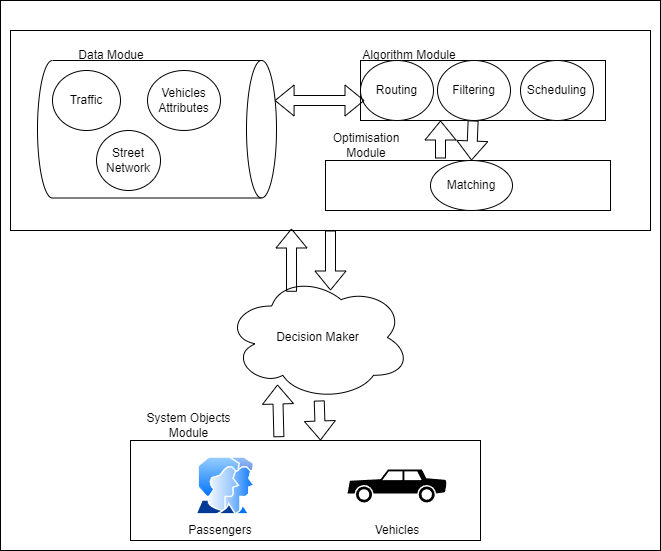
\includegraphics[width=1\textwidth]{Crest/Images/centralised_approach.png}
%     \caption{Centralised Approach to Dynamic Ride-sharing services}
%     \label{fig:centralised_approach}
% \end{figure}

% Since the centralised approach is the prevalent paradigm for handling dynamic ride-sharing problems in the literature discussed, this section discusses its essential components, which are Systems Objects, Data, Algorithms, and Optimisation. 
% The centralised approach places a single-agent decision maker at the heart of the system and includes the following modules: Systems Objects, Data, Algorithm, and Optimisation. Figure \ref{fig:centralised_approach} shows a high-level overview of the centralised approach and how its parts interact in a dynamic ridesharing system. In this strategy, each vehicle connects to a common cloud via the Internet or an intranet to take advantage of the cloud's high-performance computation and vast storage capacity. The cloud holds all necessary resources without duplication, including the street network database and optimisation programme code, among other features, and is in charge of all computations. As shown in Figure 2, when a rider submits a ridesharing request to the system, the system (decision maker) responds after updating the schedules and routes for the appropriate vehicles. The user receives a response that includes the vehicle ID and an expected pick-up time, or a rejection response if the system was unable to match a car to the request.

% \textbf{System Objects Module:}
% A ride-sharing service contains two types of objects: users and vehicles. Users use a mobile or web application to submit real-time requests to the system, which include pick-up and drop-off locations, the number of passengers, a time window for pick-up location, which specifies when the user should be picked up at the origin, and a time window for drop-off location, which specifies when the user should be dropped off at the destination. The latter two sections specify each request's limitations, which must be met in order to solve the ridesharing problem. Moreover, dynamic ridesharing problem must take into account the number of vehicles servicing over a street network (finding a vehicle for each request) by dispatching vehicles with the purpose of minimising or maximising an objective function and satisfying a set of constraints. The fleet of vehicles may vary in capacity and accessibility for certain purposes, such as wheelchair users requesting rides. The cars frequently upload their time-stamped locations to the system, allowing the decision maker to know where each vehicle is at any given time while searching for matches between vehicles and riders.

% \textbf{Data Module:} The database in the Data module contains all the required data for making ridesharing decisions, including a street network (represented as a graph or a grid) for finding routes, traffic data for handling stochasticity about travel times in the street network, and other static and dynamic data about each vehicle such as ID (static), capacity (static), current location and time (dynamic), updated schedule and route for new requests (dynamic), and number of empty seats. The Algorithm module uses the data in this database to conduct a variety of tasks, including identifying best pathways across the network, selecting candidate cars, and changing vehicle schedules when new requests are filed.

% Travel time is critical for routing, and in the absence of traffic data, less reliable routes may be discovered. Incorporating real-time traffic information leads to more optimal routes, but it is computationally expensive \cite{soa_rideshare}, hence most efforts in the literature utilise a pre-computed shortest path technique to solve the time issue. 


% \textbf{Algorithm Module:} This module consists of three submodules: routing, filtering, and scheduling. The routing submodule is in charge of calculating the best travel time between pairs of places on the street network. 


% The purpose of the filtering submodule is to efficiently choose a group of candidate vehicles capable of serving new requests while adhering to the limits of each candidate vehicle's capacity and pick-up and drop-off time windows. Obviously, going through every vehicle locally to match a travel petition when there are a lot of them is computationally unnecessary. To solve this inefficiency issue, spatial data structures such as R-tree \cite{guttman1984rtrees}, KD-tree \cite{bentley1990kdtrees}, R+-tree \cite{sellis1987rplustree}, R*-tree \cite{kriegel1990rtree}, and Quad-tree \cite{bentley1974quadtrees} have been considered. However, these data structures may not be ideal for a large-scale dynamic ride-sharing problem due to the high cost of handling vehicle dynamics and updating indices \cite{xia2003qrtree} \cite{lee2003supporting}.


% \begin{figure}[htbp]
%     \centering
%     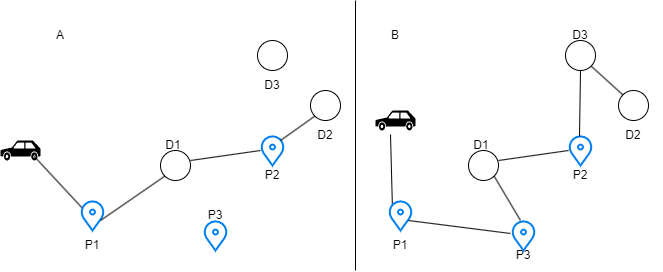
\includegraphics[width=1\textwidth]{Crest/Images/rescheduling.png}
%     \caption{An illustration of rescheduling in a dynamic ride-sharing service. (A) current route of a vehicle for serving two passengers and a new request with pick-up location P3 and drop-off location D3. (B) new route of the vehicle after rescheduling.}
%     \label{fig:rescheduling}
% \end{figure}

% The filtering submodule narrows the search space and selects a set of candidate vehicles. The scheduling submodule is then used to reschedule each vehicle's route and ensure it meets the constraints of the new request and existing rides, such as time windows for pick-up and drop-off locations. In dynamic ridesharing, a ride must begin at the pick-up site and end at the drop-off place. The routing submodule computes the shortest path between each pair of pick-up and drop-off locations. Figure \ref{fig:rescheduling} shows the scheduling submodule in dynamic ridesharing. In panel (A), a vehicle is scheduled to pick up passenger C1 at P1, drop C1 at D1, pick up passenger C2 at P2, and dump C2 at D2. When a new request with the origin P3 and destination D3 arrives, rescheduling is required. Panel (B) depicts the results of rescheduling, a new route, and the order in which passengers are served.

% The rescheduling problem can be addressed in one of two ways: (i) Insert the new request at any point in the current schedule without changing the order of the existing places; this is known as the insertion heuristic approach. To add a new request to the current route with n stops (pick-up and drop-off sites), there are (n+1) (n+2)/2 scheduling options. This method is frequently utilised in the literature \cite{huang2013large} \cite{coslovich2006twophase} \cite{jaw1986heuristic} because to its low computational cost. (ii) create a completely new schedule and solve an open-loop TSP (Travelling Salesman Problem) with a computationally expensive time frame (O(n!)).


% \begin{figure}[htbp]
%     \centering
%     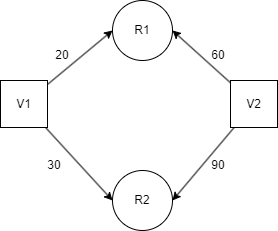
\includegraphics[height=6cm]{Crest/Images/queuing.png} % Adjust the height as needed
%     \caption{An example of queueing approach in ride-sharing problem. The numbers on links are travel times for vehicles-requests \cite{ayala2018spatio}.}
%     \label{fig:queuing}
% \end{figure}


% \textbf{Optimisation Module:}The optimisation module finds an optimal solution to the problem by selecting the candidate vehicle that best meets the request from all of the candidates evaluated by the scheduling submodule for contribution to the objective function. The optimisation module is at the heart of a ride-sharing solution, executing a matching function that assigns vehicles to requests with the goal of optimising an objective function. When determining ride-sharing matches, the models take into account one or a weighted mixture of the following cost functions. \cite{agatz2012optimization}: reducing overall distances or travel times by all cars on the street network; minimising vehicle detours; minimising passenger costs; and maximising the number of successful ride-share requests. These objective functions take into account a range of limitations, including vehicle capacity, user-specified departure or drop-off times, and trip costs. 

% The assignment task is determined by how the optimisation issue handles incoming requests. Essentially, there are two study approaches to addressing the assignment problem: queueing (first-come, first-served) and batch assignment. The queueing strategy, commonly used for solving assignment problems, prioritises all trip requests in chronological order. It should be noted that this is a greedy method that may not produce a global optimal solution because it does not take into account all of the conceivable combinations of shared trip petitions. Using the queuing method shown in Figure \ref{fig:queuing}, request 1 comes before request 2 and vehicles can not handle both at the same time. The optimisation module gives vehicle 1 to request 1, which costs 20, and vehicle 2 to request 2, which costs 90, for a total cost of 110. According to \cite{ayala2018spatio}, this type of vehicle-request assignment matches Nash equilibrium \cite{nash1950equilibrium}. In the scenario in \ref{fig:queuing}, assigning request 1 to vehicle 1 is the best option for vehicle 1 because its travel time to request 2 is longer. Vehicle 2 cannot get request 1 to reduce its trip time because vehicle 1 is closer to request 1. In this case, the vehicles act selfishly for their personal gain rather than attempting to optimise overall performance. While the queuing strategy is effective at tackling the underlying combinatorial optimisation problem, it sacrifices optimality. 

% \begin{figure}[htbp]
%     \centering
%     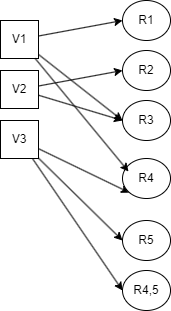
\includegraphics[height=6cm]{Crest/Images/batch_assignment.png}
%     \caption{ An example of batch assignment }
%     \label{fig:batch_assignment}
% \end{figure}

% Figure \ref{fig:queuing} shows that the Nash equilibrium assignment is not optimal. By matching vehicle 2 to request 1 and vehicle 1 to request 2, a better solution with a total cost of 90 is possible. This ideal plan is only possible if incoming requests are aggregated and then allotted to all vehicles within a defined interval. The goal of the batch assignment strategy shown in Figure \ref{fig:batch_assignment} is to compute the optimal assignment of requests to vehicles that minimises or maximises the objective function. Note that each vehicle may be able to handle a group of requests simultaneously; therefore, more nodes will be added to the bipartite graph depicted in Figure \ref{fig:batch_assignment}. Obtaining a close-to-optimal solution in a large-scale dynamic ridesharing situation is the primary rationale for using the batch assignment technique over the queuing strategy, despite the fact that the batch assignment approach is an NP-hard problem. This suggests that heuristics and/or approximate approaches can provide a solution to this large-scale combinatorial optimisation problem in a fair amount of time \cite{liebling1987large}. 

% \subsection{Dynamic Ride-sharing}
% \begin{table}[ht]
% \centering
% \caption{Analogy between dynamic ridesharing problem and different VRP variants.}
% \label{tab:vrp_variants}
% \renewcommand{\arraystretch}{1.5}
% \resizebox{\textwidth}{!}{%
%     \begin{tabular}{|l|c|c|c|c|}
%     \hline
%     \textbf{Problem} & \textbf{Dynamism} & \textbf{Vehicle's capacity} & \textbf{Paired pick-up and drop-off} & \textbf{Time window} \\ \hline
%     \textbf{Dynamic Ridesharing} & \checkmark & \checkmark & \checkmark & \checkmark \\ \hline
%     \textbf{DVRPTW} & \checkmark & \checkmark & & \checkmark \\ \hline
%     \textbf{MTSPTW} & & \checkmark & & \checkmark \\ \hline
%     \textbf{DPDP} & \checkmark & & \checkmark & \\ \hline
%     \textbf{DDARP} & \checkmark & & \checkmark & \checkmark \\ \hline
%     \end{tabular}%
% }
% \end{table}

% \begin{figure}[htbp]
%     \centering
%     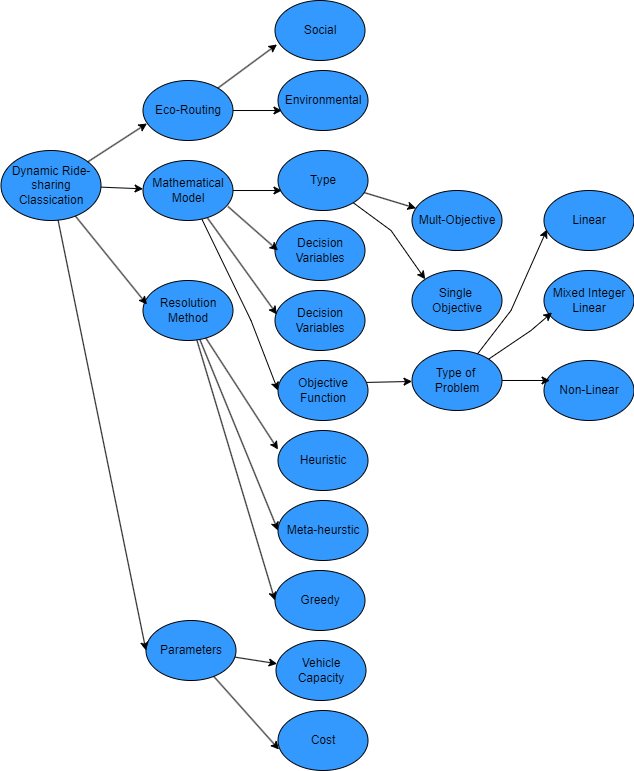
\includegraphics[width=1\textwidth]{Crest/Images/vrp_classification.png}
%     \caption{A systematic review of Dynamic Ride-sharing presented in this literature}
%     \label{fig:vrp_classification}
% \end{figure}

% To further understand the dynamic ride-sharing problem, it is helpful to review prior literature on solutions. The literature on this topic is extensive\cite{Pillac2013DVRPSurvey}, necessitating a focused understanding of the key themes to be addressed when reviewing it. Figure \ref{fig:vrp_classification} presents a systematic overview of these topics, providing a framework for discussion that aligns with the scope of this research. 

% There are several types of solution approaches to the dynamic VRP, including dynamic vehicle routing problem with time window (DVRPTW), dynamic pick-up and delivery problem (DPDP), dynamic dial-a-ride problem (DDARP), and multiple travelling salesman problem with time window (MTSPTW). Table \ref{tab:vrp_variants} compares various kinds of VRP to the dynamic ridesharing problem. It is possible to use the solution to the classic DDARP problem to solve the dynamic ridesharing problem because the two problems are mathematically similar and have similar constraints. These constraints are: a) vehicles with limited capacity; b) passenger requests with a pair of pick-up and drop-off locations; and c) passenger requests with time windows for pick-up and drop-off locations \cite{meng2021dynamic}. The DVRPTW routes begin and stop at a depot, where the concept of pick-up and delivery points is introduced \cite{abdulaal2017solving}. The MTSPTW seeks to find a set of optimal vehicle routes within a certain time frame. In this sort of problem, the concept of dynamism does not exist, the vehicle capacity limitation is released, and, similarly to DVRPTW, the paired pick-up and drop-off site constraint is released \cite{soa_rideshare}. The DPDP approach is appropriate for issues in which requests are made for the delivery of objects such as parcels or letters, time windows are not tight, and capacity limitations do not exist \cite{zhao2021research}. The main idea behind the DDARP is that vehicles start and end their routes at different depots (or the same depot), users' requests are broadcast during the operation, and users must be moved between pairs of pick-up and drop-off locations. The goal is to find the best routes for vehicles that minimise distance while meeting constraints like time windows for each request \cite{thiago19lastmile}. The DDARP allows vehicles to arrive at pick-up sites before the start of the time window but no later than the end of the time window. By example, this holds true for the pick-up and drop-off time windows limitation in the dynamic ridesharing problem. In this context, the dynamic VRP with time windows (DVRPTW) is particularly relevant \cite{meng2021dynamic}. Ride-sharing services must account for dynamic trip requests that arrive in real time, with passengers specifying their pick-up and drop-off times. The system must then allocate vehicles in a way that maximises service efficiency while minimising waiting times and detours\cite{dynamic2024model}. Several factors contribute to the growth of ride-sharing services, including the demand for lower travel costs, concerns about environmental sustainability, and the advancement of connected and autonomous car technologies. Modern ride-sharing services like Uber, Lyft, and BlaBlaCar have proved the power of technology in tackling transportation inefficiencies, but there are still problems in scaling these systems for widespread usage, particularly in urban areas\cite{bakibillah2021incentive}. Adding EVs into the mix introduces further complexity, as the problem must also consider charging schedules and energy consumption \cite{abdulaal2017solving}. Because of the tight relationship between the DVRPTW problem and the DDARP, the remainder of this section focuses on literature that suggest novel techniques for solving variants of the dynamic ride-sharing problem. 

% In \cite{dastpak2021off}, the authors develop a stochastic form of the VRP called the Vehicle Routing Problem with Stochastic Customers and Demands (VRPSCD). In this paradigm, both passenger locations and destinations are unknown at the planning stage. The stochastic information is exposed in two stages: first, customer locations and expected requests are known at the start of the day, and second, actual customer demands are monitored during visits. This challenge is similar to real-world circumstances such as parcel delivery and rubbish collection, in which consumer expectations and locations are unknown until just before service. The VRPSCD's goal is to maximise overall demand supplied within a given time frame, allowing vehicles to return to the depot for preventive replenishment before their capacity is reached. To address this issue, the authors \cite{dastpak2021off} offer a decentralised solution that employs a Markov Decision Process (MDP), allowing vehicles to make autonomous judgements based on real-time data.

% The operational issues of dynamic ride-sharing originate from the engagement of various parties with competing objectives, such as private corporations looking to maximise revenue, governments looking to reduce congestion and pollution, and passengers looking for quick and inexpensive transportation. A greater understanding of the intricate relationships between various parties may result in more successful ride-sharing systems \cite{xie2020optimal} \cite{soa_rideshare}.

% The study \cite{baudru2024comparative} focusses on Peer-to-Peer (P2P) ride-sharing, which leverages private vehicles to pool many passengers with similar itineraries and offers a flexible and low-cost mobility alternative.

% Ride-sharing services can be centralised (big, open groups) or decentralised (small, closed groups), with vehicles owned by one or more ride-sharing participants\cite{houerbi2023blockchain}. Despite ride-sharing's effectiveness in lowering the number of vehicles on the road and associated costs, substantial obstacles persist, particularly in optimising for the preferences of both passengers and drivers \cite{houerbi2023blockchain}. Conflicting aims, such as reducing driving detours and passenger wait times, make it impossible to fulfil all preferences at once \cite{joseph2021blockwheels}.

% This study \cite{baudru2024comparative} compares several strategies for organising ride-sharing groups, including execution time, percentage of satisfied requests, driver detours, and passenger waiting times. The authors present a model to predict user demand based on car usage data from Belgium, allowing them to evaluate multiple user grouping strategies, including OD Similarity, OD Clustering, and Trip Similarity.

% The study emphasises \cite{baudru2024comparative} the economic and environmental benefits of lowering road traffic, stating that inefficient urban mobility costs billions of dollars each year in both the EU and the United States, and that road transport contributes significantly to carbon emissions and urban air pollution. 

% This study \cite{ghandeharioun2023rideshare} examines the operational assignment problem in on-demand ride-sharing services. It aims to model stakeholder objectives and propose policies that provide efficient and mutually beneficial solutions. A real-time simulation framework is created to model dynamic supply-demand matching while accounting for user-specified tolerance times. The optimisation problem is solved with both heuristics and commercial solvers, allowing for quick, efficient decision-making and providing insights into how to improve ride-sharing system operations.



% Dynamic ride-sharing services confront real-time optimisation issues, including the requirement for efficient ride-matching algorithms. In \cite{optimiserideshare}, the authors focus on dynamic ride-sharing from the perspective of sharing cost mechanisms, including uncertainty in trip petitions. Their algorithm assesses various re-optimisation rates, such as when a new trip petition arrives or at predetermined intervals. The method becomes more difficult due to the uncertainty of trip requests, which can be filed anywhere from a few minutes to a few hours before departure. The overall distance travelled or total travel time for each individual ride serve as the optimisation criteria in this scenario. This approach views drivers as private individuals, which means that vehicle availability is linked with their own travel requirements.

% The ride-sharing problem is commonly represented as a Pickup and Delivery Problem with Time Windows (PDPTW), which is known to be NP-hard \cite{nphardness2024wikipedia} \cite{herbawi2012modeling}. The complexity of handling this problem grows with the amount of requests, hence, it is critical to design effective and scalable techniques to handle the high frequency of ride-sharing requests. \cite{zhong2024wait}.

% To overcome the scalability issues in centralised ride-sharing, this work \cite{alisoltani2022spacetime} presents a clustering-based strategy to increase the efficiency and scalability of matching algorithms. The approach provides a "shareability function" (SF) that assesses the likelihood of two trips being shared, taking into account both parallel and sequential sharing possibilities. The SF calculates the additional travel time required to share trips vs serving each trip individually, allowing the clustering algorithm to combine trips with high shareability potential.

% Another study \cite{wallar2019optimizing} proposes a method to estimate the optimal number of vehicles needed to fulfil all travel demand in a city while preserving acceptable waiting times and delays. This offline technique informs fleet operators on the fleet size and vehicle distribution required to fulfil historical demand. The study demonstrates that optimising fleet size and distribution can greatly increase the efficiency of MoD systems, allowing for more effective and strategic fleet management.

% Another key problem is to maintain high service availability. \cite{hafiz2020flexible} focuses on providing real-time scheduling for ride-sharing journeys. They suggest a strategy for reassessing ride-matching over time, clustering passengers and drivers in the same neighbourhood to maximise viable trip options. Their approach ensures a ride back for consumers who have previously received an outbound trip, alleviating concerns regarding trip reliability and return journeys. This ensures a certain level of service quality, as passengers may be confident that once allocated to a journey, they will be able to finish their return trip without further complications.

% Ride-sharing has also been explored as part of multi-modal transportation systems, particularly in last-mile transportation. In \cite{thiago19lastmile} and \cite{zeng2020exploring}, the authors examine dynamic ride-sharing integrated with public transport for the last-mile of a commute. Their work considers the routing of passengers who have reached a central station using public transportation and are now dispersing to their final destinations. The goal is to minimise the number of vehicles on the road by efficiently allocating passengers to available vehicles, thereby reducing congestion and improving travel efficiency.



% Moreover, with the global shift towards sustainable energy, integrating EVs into ride-sharing services has become increasingly important. However, privacy and trust concerns often impede the broader adoption of ride-sharing services. The authors of \cite{Reference4} address these concerns by proposing a co-utilisation framework based on game theory. In their approach, all involved parties must benefit from participating in the ride-sharing service, ensuring mutual trust among passengers and drivers. This framework seeks to reduce travel costs for passengers while also decreasing the number of vehicles on the road and mitigating traffic congestion. Their approach highlights how privacy and trust mechanisms can be integrated into dynamic ride-sharing systems to improve user confidence.

% In summary, while dynamic ride-sharing offers significant benefits, such as reduced congestion, lower emissions, and cost savings, the challenges of real-time optimisation, service reliability, and trust remain crucial to its success. The integration of EVs offers additional opportunities for making ride-sharing more sustainable and widely adopted in urban environments\cite{mamalis2019ridesharing}.

% Eco-routing introduces a variant of DVRP known as Green Vehicle Routing Problem(GVRP). The literature on GVRP is currently developing, with contributions focusing on topics such as reverse logistics, recycling, and emissions management. \cite{lin2014survey} identified research gaps between VRP and Green Logistics, notably the use of time-dependent VRP to reduce emissions during transport. According to studies \cite{salimifard2012green} and \cite{asghari2021green}, integrating environmental costs into VRP is still in its early stages, despite its potential. This work \cite{lin2014survey} adds to the field by doing a comprehensive evaluation of GVRP literature and identifying future research objectives. It provides useful insights for academic studies and practical applications by categorising GVRP variants and exposing gaps in existing research. Governments, non-profit organisations, and corporations can utilise GVRP models to assess the social, environmental and cost implications of transportation plans and take steps towards more sustainable logistics operations. It tries to reduce greenhouse gas emissions and other pollutants produced by transportation systems. It is part of the larger idea of ITS, in which information and communication technology (ICT) plays an important role in optimising different transportation aspects including as speed, route guidance, and traffic signals in order to reduce environmental effect. Eco-routing adds environmental objectives, such as decreasing emissions, whereas traditional vehicle routing models largely focus on minimising journey time \cite{alfaseeh2020multi}.

% Eco-Routing models can be categorised into four aggregation levels\cite{alfaseeh2020multi}:
% \begin{enumerate}
%     \item \textbf{Microscopic (I)}: These models have excellent spatial and temporal resolution, allowing for precise estimations of traffic and emission indicators. However, the trade-offs include longer calculation times, more resource utilisation, and higher input data needs.
    
%     \item \textbf{Macroscopic (A)}: This thesis focusses on macroscopic models that have coarser spatial and temporal resolutions\cite{gridmap}. These models are less precise than microscopic models, but they are easier to use and effective when high-resolution data is unavailable. Macroscopic models are suitable for large-scale situations when simplicity and computing economy are important.

%     \item \textbf{Mesoscopic (E)}: These models strike a balance between microscopic and macroscopic models, with medium levels of spatial and temporal resolution. Despite their potential benefits, none of the reviewed studies applied mesoscopic models for traffic flow and emissions in the context of eco-routing.

%     \item \textbf{Mixed aggregation (M)}: This category includes multiple levels of aggregation for traffic and emission models in order to optimise both.
% \end{enumerate}
% The basic purpose of eco-routing is to steer vehicles along the most energy-efficient routes in order to optimise fuel use and eliminate harmful emissions like GHG \cite{naeem2024energy}. The dynamic End-to-End (E2E) routing system utilises a network of intelligent intersections and CAVs as a famous example of distributed routing. This system uses technologies such as Dedicated Short-Range Communication (DSRC) and 5G to allow for real-time communication between vehicles and infrastructure \cite{djavadian2020multi}. The intelligent junctions collect and communicate real-time traffic data, allowing them to direct CAVs to their destinations while taking into account current network conditions.



% Studies \cite{djavadian2020multi} and \cite{alfaseeh2019multi} have demonstrated that E2E CAV routing systems can reduce travel time and enhance network throughput, especially under high market penetration rates (MPR) and heavy congestion. However, while travel time optimisation alone has shown some potential to reduce emissions, the full benefits of eco-routing may only be realised by explicitly incorporating emission reduction objectives into the routing algorithms. 

% In \cite{ham2021routeoptimise}, the authors present a unique approach to the E-VRP with Time Windows (E-VRPTW) by including Time-of-Use (TOU) electricity pricing, where retail electricity prices fluctuate hourly based on wholesale market circumstances. By intelligently changing vehicle charging to off-peak periods, significant cost reductions can be accomplished. For example, shifting charging from 8 pm to 4 am leads in a 68\% reduction in electricity expenditures. The goal is to reduce not only energy prices, but also the number of EVs utilised and overall journey distance. By incorporating TOU pricing into the E-VRPTW model, this study makes a substantial contribution to cost-efficient routing of electric AV fleets, opening up new possibilities for optimising both transportation and energy management in the developing autonomous taxi business. 

% Heuristics and metaheuristics like genetic algorithms, simulated annealing, and particle swarm optimisation are often used to solve VRP and its variants\cite{kedia2017review}. Exact methods like mixed-integer programming (MIP) are also sometimes used\cite{zuo2017using}. More recent work has explored machine learning-based methods to enhance route optimisation\cite{ren2023solving} \cite{alduoli2018hybridizing}.

% The authors \cite{dastpak2021off} create a Q-learning method, DecQN, to solve the VRPSCD. This reinforcement learning system allows vehicles to learn optimal policies through simulation, and modern techniques such as Replay Memory and Double Q Networks have increased the algorithm's efficiency. DecQN beats benchmark policies for VRPSCD and is competitive with cutting-edge approaches for VRP with Stochastic Demands (VRPSD), despite not being especially designed for that challenge.



% The aforementioned approaches can be used to find solutions to small and medium size 
% instances of the ride-sharing problem in a reasonable amount of time; however, there are some areas for further examination. First, the applicability of the proposed techniques to deal with large-scale 
% optimisation problem with a high degree of dynamism, explained earlier, need to be investigated. 
% Second, in all cases, a queuing approach has been used in serving the new requests; see Section 
% 2.1.4 for a discussion of the pros and cons of this approach. Third, the quality of solutions in these 
% approaches is not known, i.e., how far the objective value of a solution is from the optimal value


% \section{Smart Energy Community based Ride-sharing for Autonomous Electric Vehicles}
% SECs are decentralised energy networks in which local entities (households, companies, and public infrastructure) generate, store, and use renewable energy. These communities rely on distributed energy resources (DERs) such as solar panels, wind turbines, hydro power and battery storage devices to achieve energy independence and sustainability \cite{kahlen2018electric}. SECs are critical to achieving a low-carbon energy future because they optimise local energy production and consumption, reduce reliance on nonrenewable energy sources, and improve grid resilience \cite{vanSummeren2019community}.

% The integration of autonomous electric vehicles (AEVs) into Smart Energy Communities (SECs) has the potential to optimise mobility and energy management \cite{song2023electric} \cite{satoya2014community}. AEVs, as part of shared mobility in Mobility-on-Demand (MoD) networks, can not only meet transportation demands but also contribute to the energy grid using vehicle-to-grid (V2G) technology\cite{dapuzzo2022smart}.The study \cite{kahlen2018electric} found that the mixed rental-trading strategy improves energy markets, fleet owners, and the environment. Integrating EVs into the energy market can lower energy prices by 3.4\%, reduce renewable energy curtailment by 97\%, and enhance earnings for fleet owners by 4.3\%. Sharing transportation services have problems like fleet rebalancing, which happens when EVs gather in areas with high demand at certain times. Adding AEVs that can connect to V2G networks is a way to fix these problems. AEVs have the ability to store excess renewable energy generated by SECs during times of low transportation demand. This allows them to return the energy to the grid when it is required, achieving a balance between the supply and demand of energy. Having this dual capability allows for the optimisation of vehicle availability while also contributing to grid stability through energy redistribution, which ultimately results in a transportation system that is more environmentally friendly and efficient \cite{Reference104}.

% Collaboration between SECs and EV fleets benefits ride-sharing services in particular. By synchronising EV charging with the availability of renewable energy in the community, SECs can ensure that electric vehicles are charged during peak renewable generation periods, such as throughout the day when solar energy is available \cite{piazza2021smartev}. This strategy decreases reliance on fossil fuels for charging and lowers the carbon impact of transport services\cite{fesciogluunver2023electric}. Furthermore, proactive management of EV charging schedules helps to avoid overloading the local grid and ensures that charging occurs when energy prices are lower, increasing the cost-effectiveness of ride-sharing services\cite{wang2016charging} .

% As EV use grows, their batteries can function as distributed energy storage units in SECs. This allows fleet owners to participate in power markets by leveraging spare battery capacity to absorb excess electricity during low consumption periods and discharge it at high demand \cite{spoorthi2022review} \cite{chen2020real}. The paper \cite{vanSummeren2019community} proposes a combined rental-trading model for fleet owners in which EVs are employed for both automobile rentals and energy trading. By treating the fleet as a source of energy, the technique helps optimise when to charge or discharge EVs in response to variable electricity prices.

% The research \cite{kahlen2018electric} collects real-time data on battery levels and EV positions using GSM and GPS. The technique is validated with real-world data from car-sharing fleets in several cities, such as San Diego, Amsterdam, Stuttgart, and Copenhagen. The strategy interacts with Northern Europe's Nord Pool Spot power market, replicating market dynamics as EV fleet owners bid to charge or discharge electricity.


% A significant gap in existing literature is the lack of attention for the variety of charging facilities in EVCSs. In fact, EVCSs often have a variety of charging facilities to satisfy a wide range of customer needs, including slow, regular, and fast charging \cite{afshar2020literature}. This complexity necessitates an effective strategy for optimising the planning of EVCSs with mixed charging facilities.

% The study \cite{luo2018optimal} offers a new optimisation model to minimise the total annualised societal cost of the EV charging system. This cost covers the initial investment, grid reinforcement, operations and maintenance, and network losses. The model uses a Monte Carlo simulation \cite{montecarlo2024wikipedia} to estimate the distribution of charging demands among various types of facilities. To solve the difficult optimisation model, a two-step equivalence and an exact Second-Order Cone Programming (SOCP) relaxation are employed to convert the problem into a Mixed Integer SOCP (MISOCP), which can be effectively solved with commercial solvers.

% Uncoordinated EV charging in an SEC setting may cause grid instability. The study \cite{mao2019energymanage} investigates the potential of smart scheduling strategies to overcome these challenges, avoiding costly infrastructure changes and optimising EV charging to benefit both the power grid and EV users. 

% The study \cite{mao2019energymanage} presents a unique Intelligent Scatter Search (ISS) algorithm architecture to address these difficulties. The ISS framework uses scatter search and sequential quadratic programming (SQP) to manage both unidirectional and bidirectional vehicle-to-grid (V2G) charging scenarios, allowing for variable and steady power rates. This technique is intended to be a complete and universal solution that accommodates a variety of EV charging modes and rates while also meeting current and future smart grid needs.

% Integrating EVs into SECs is crucial for promoting the concept of the "energy citizen." This notion involves people actively engaged in energy generation, use, and management in their own communities \cite{barone2020sec}. Individuals/Communities who own and operate EVs that interact with SECs can help their communities achieve overall energy autonomy while saving money and reducing carbon emissions\cite{boasso2021sec}. This is consistent with broader policy objectives, such as those specified in the European Green Deal, which encourages carbon-neutral cities and sustainable transport networks\cite{greendeal}.

% SECs' decentralised and collaborative concept, along with EV integration, provides a resilient and adaptive infrastructure that is well-suited to the changing demands of modern urban mobility. As cities grow and the transportation sector transitions to electric and self-driving vehicles, SECs' role in promoting sustainable, carbon-neutral transportation systems will become increasingly more important. This collaboration between energy and transport systems marks a big step towards creating smart, sustainable cities capable of meeting the problems of climate change and urbanisation.

